\documentclass[a4paper, titlepage, appendixprefix, numbers=noendperiod]{scrreport}

% % % % % % % % % % % % % % % % %
% WICHTIG!
% Das Dokument ist zweiseitig formatiert, es MUSS beidseitig gedruckt werden.
% Neue Kapitel beginnen immer rechts (Option openright)
% wird "numbers=noendperiod" gelöscht, reagiert das KOMASkript Dudenkonform: bei Überschriftennummerierung keine Endpunkte ohne Anhang; mit Endpunkten, wenn es einen Anhang gibt 
% % % % % % % % % % % % % % % % %

% Laden der Zusatzpakete (aus dem Ordner "input") 
% Paket für Input Encoding
% wenn utf8 nicht funktioniert, bitte ansinew (Windows) oder applemac (Mac) benutzen.
\usepackage[utf8]{inputenc}

% Font Encoding, u.A. für die korrekte Ausgabe in PDF-Dokumenten
\usepackage[T1]{fontenc}

% Anpassung der Sprache, in diesem Fall: Deutsch in neuer Rechtschreibung
\usepackage[english]{babel}

% Einstellung der Geometry des Layouts
\usepackage[textwidth=145mm,textheight=235mm,left=35mm,top=25mm,headsep=5mm]{geometry}

% optimierte Schrift für PDF-Dokumente
\usepackage{lmodern}

% Zum einfachen Einfügen von Grafiken
\usepackage{graphicx}

% Für lang Tabellen
\usepackage{longtable}

% Erweiternde Pakete für den Formelsatz
\usepackage{amsmath, amssymb, amsthm, amsfonts}

% Erstellt Verweise in PDF-Dokumenten. Die Verweise haben die Farbe schwarz, sind also nicht extra gekennzeichnet.
\usepackage[colorlinks,linkcolor=black,citecolor=black]{hyperref} 

% Paket für Aufzählungen. Zu verwenden wie itemize.
\usepackage{enumerate}

% Anführungszeichen
\usepackage[style=german]{csquotes} 

% "schöne" Tabellen
\usepackage{booktabs}

% Deckblatt für die Seminararbeit. Metadaten in titlepage.tex anpassen.
\usepackage{VOSTitle}

% Paket für die Selbstständigkeitserklärung, nutzt die Metadaten in titlepage.tex
\usepackage{VOSStatement}

% Für Zeilenabstände
\usepackage{setspace}

% Blindtext
\usepackage{lipsum}

% Paket für das Abkürzungsverzeichnis
\usepackage{acronym}

% Paket für die Zusammenfassung nach dem Titelblatt
\usepackage[style]{abstract}

% Paket für angepasste Bibliografie-Stile
\usepackage{bibgerm}

\usepackage{fancyhdr}
% Optional: Gleitobjekte nicht in andere Abschnitte fließen lassen 
%(Doku:http://mirror.informatik.uni-mannheim.de/pub/mirrors/tex-archive/macros/latex/contrib/placeins/placeins-doc.pdf) 
%\usepackage{placeins}

\usepackage[style=apa]{biblatex}
\usepackage{parskip}

% Laden weiterer Einstellungen
% einige andere Einstellungen oder Ergänzungen

% Festlegen des Titel-Stils der abstract-Umgebung
\renewcommand{\abstitlestyle}[1]{{\Large\bfseries\sffamily\noindent #1}\hfill}

% Änderung der Nummerierung der Formeln	
\numberwithin{equation}{section} 

% anderthalbfacher Zeilenabstand 
\onehalfspacing

% Globaler Seitenstil

\pagestyle{headings}
\fancyhf{} %
\pagestyle{fancy} %
\fancyfoot[LE,RO]{\thepage} %
\fancyhead[LO]{\nouppercase\rightmark} %
\fancyhead[RE]{\nouppercase\leftmark}%




% Parameter für das Titelblatt und die Selbstständigkeitserklärung
% % % % % %
% Bitte beachten Sie die Hinweise zum Ausfüllen.
% % % % % % 

% Lehrstuhl, an dem die Arbeit geschrieben wurde
\professur{Chair of Econometrics and Statistics}

% Art der wissenschaftlichen Arbeit
\thesistype{Diploma Thesis}

\fak{\enquote{Friedrich List} Faculty of Transport and Traffic Sciences}

% Namen und Matrikelnummern möglicher Autoren.

% % % % % % % % % % % % % % % % % % % % % % % % % %
%   Bitte die Autoren DER REIHE NACH auffüllen	  %
% % % % % % % % % % % % % % % % % % % % % % % % % %

% Bei nur einem Autor muss authorOne ausgefüllt werden
\authorOne{Henry Haustein}
\matrikelAuthorOne{4685025}

% Hat die Arbeit zwei Autoren, muss authorTwo ausgefüllt werden
\authorTwo{} 
\matrikelAuthorTwo{}

% Bei drei Gruppenmitgliedern ist auch authorThree zu belegen
\authorThree{} 
\matrikelAuthorThree{}

% NUR, FALLS TATSÄCHLICH BENÖTIGT, ANSONSTEN LEER LASSEN
% Für das vierte Gruppenmitglied
\authorFour{}
\matrikelAuthorFour{}

% Titel der Aufgabenstellung
\title{WIP}

% Betreuer am Lehrstuhls
\betreuer{Haozhe Jiang}

% Datum der Abgabe. \today ist der heutige Tag, bitte ggfs. ändern auf den 8. Januar oder wann immer Sie abgeben
\date{XX.XX.XXXX}


%\bibliography{library}
\addbibresource{library.bib}

% % % % % % % % % % % % % % % %
% Beginn der document-Umgebung
% % % % % % % % % % % % % % % %
\begin{document}

% Erstellen des Titelblatts
\maketitle

\cleardoublepage

% Umstellung der Seitennummerierung auf römische Ziffern
\pagenumbering{roman}

% Zusammenfassung, wenn nicht benötigt, auskommentieren!
% \selectlanguage{ngerman}

% \begin{abstract}
% \noindent
% \lipsum[20-21]
% \end{abstract}

% FALLS BENÖTIGT: Englische Zusammenfassung (in der Regel nicht in Seminararbeiten gefordert!)
%\selectlanguage{english}
%\begin{abstract}
%\noindent
%\lipsum[20-23]
%\end{abstract}
%\selectlanguage{ngerman}

% \cleardoublepage

% Erstellen des Inhalts-, Abbildungs- und Tabellenverzeichnisses
\tableofcontents
\cleardoublepage
  
\phantomsection\addcontentsline{toc}{chapter}{List of Figures} 
\listoffigures
\cleardoublepage

\phantomsection\addcontentsline{toc}{chapter}{List of Tables}
\listoftables
\cleardoublepage

% Einfügen des Abkürzungsverzeichnisses
% Bitte die Datei listofabbreviations.tex im Order um die eigenen Abkürzungen ergänzen.
% \phantomsection\addcontentsline{toc}{chapter}{Abkürzungsverzeichnis}
% \chapter*{Abkürzungsverzeichnis}
% Der String XXXXXXXX hat keine wirkliche Bedeutung; die acronym-Umgebung verlangt einen Parameter, der angibt, wie breit die Abkürzungen in der Übersicht sein dürfen, in diesem Fall 8*X
\begin{acronym}[XXXXXXXX]
% \acro{BIP}{Bruttoinlandsprodukt}
% \acro{x}[\ensuremath{\bar{x}}]{Mittelwert}
\end{acronym}
% \cleardoublepage

% Umstellung der Seitennummerierung auf wieder auf arabische Ziffern 
\pagenumbering{arabic}

% Hier beginnen die Kapitel und der eigentliche Inhalt.
% Es empfiehlt sich, den Inhalt einzelner Kapitel in separaten Dateien zu halten und diese hier mit \input{file} einzubinden.

%Einleitungskapitel, hier sind derzeit noch nachfolgende Kapitel drin, diese besser in eigene Dateien trennen
% \section{Introduction}
\label{sec:introduction}

- In vielen Einführungsvorlesungen in Finance wird die Annahme getroffen, dass Renditen am (Aktien-)Markt normalverteilt sind. Diese Annahme ist jedoch nicht korrekt, da empirische Untersuchungen zeigen (z.B. Mandelbrot 1997), dass Renditen oft nicht normalverteilt sind. So sind Renditen oft leptokurtisch, d.h. die Verteilung hat dickere Enden als die Normalverteilung. Zudem sind Renditen oft schief, d.h. die Verteilung ist nicht symmetrisch. Diese Eigenschaften sind wichtig, da sie die Risikobewertung und das Risikomanagement beeinflussen.
- Die Idee der normalverteilten Renditen kommt von Bachelier (1900), der die These aufstellte, dass der Preis eines Assests sich wie eine Brownian Motion verhält. Diese These wurde von Black, Scholes und Merton im Jahr 1973 weiterentwickelt zum Black-Scholes-Merton-Modell, welches die Finanzwelt revolutionierte (Heimer & Arend 2008). Der britische Mathematiker Ian Steward is sogar der Meinung, dass dieses Modell verantwortlich für die Finanzkrise 2007-2008 war (Steward 2012).
- Die Schwächen des Black-Scholes-Modells sind die Annahmen über unter anderem eine konstante Volatilität und eine normalverteilte Rendite. Diese Annahmen sind empirisch nicht haltbar, da die Volatilität oft nicht konstant ist und die Renditen oft nicht normalverteilt sind. Daher wurden Modelle entwickelt, die diese Schwächen adressieren. Eines dieser Modelle ist das Heston-Modell, welches von Heston (1993) vorgestellt wurde. Das Heston-Modell ist ein stochastisches Volatilitätsmodell, d.h. die Volatilität ist nicht konstant, sondern folgt auch einem Zufallsprozess. Das Heston-Modell ist ein beliebtes Modell in der Finanzmathematik, da es die Schwächen des Black-Scholes-Modells adressiert und die empirischen Eigenschaften von Renditen besser abbildet.
- Das Heston-Modell hat keine geschlossene Lösung mehr, im Gegensatz zum Black-Scholes-Modell, daher müssen numerische Verfahren zur Lösung des Modells verwendet werden. Diese Verfahren sind aufwendig, entweder simuliert man viele Pfade oder man nutzt die charakteristische Funktion in Kombination mit einer inversen Fourier-Transformation, um eine Preisverteilung zu berechnen. Diese Preisverteilung kann dann genutzt werden, um Optionen zu bewerten (Gatheral 2011).
- Das setzt voraus, dass man bereits die Parameter des Modells kennt. Man kann das Modell an den Markt anpassen, indem man es als Least-Squares-Problem definiert, wobei die Zielfunktion ist, die Preise am Markt zu reproduzieren. Normalerweise nimmt man die Preise von vanilla options (Floc'h 2018) oder von variance swaps (Guillaume & Schoutens 2013).
- Da Verteilung der Renditen doch recht ähnlich zur Normalverteilung ist, ist es das Ziel der Arbeit zu untersuchen, inwiefern sich Expansionsverfahren für die Normalverteilung, wie z.B. die Gram-Charlier Expansion (Gram 1883, Charlier 1914) genutzt werden kann die Normalverteilung zu verändern, um die Renditen des simulierten Heston-Modells abzubilden. Dazu wird das Heston-Modell mittels Andersens (2008) QE-Verfahren für einen großen Parameterraum simuliert, Momente und Kumulanten berechnet und dann die Expansionsverfahren angewendet. Die Ergebnisse werden dann mit der theoretischen Dichte verglichen, um zu sehen, wie gut die Expansionsverfahren die Dichte approximieren können.

- Die Arbeit gliedert sich in die folgenden Bereiche: Im Kapitel \ref{sec:heston_model} wird das Heston-Modell vorgestellt, das Kapitel \ref{sec:moments} werden Grundlagen zu Momenten und Kumulanten gelegt und auf die Berechnung dieser bei Hochfrequenz-Handelsdaten eingegangen. Im Kapitel \ref{sec:expansion_methods} werden die Expansionsverfahren vorgestellt und in Kapitel \ref{sec:methodical_approach} die praktische Umsetzung der Arbeit erläutert. Es folgt Kapitel \ref{sec:results} mit Ergebnissen und die Arbeit schließt mit Kapitel \ref{sec:conclusion} ab, wo die Arbeit zusammengefasst und ein Ausblick gegeben wird.

%Anhang
% \appendix
% \phantomsection\addcontentsline{toc}{chapter}{Appendices}
\section{Introduction}
\label{sec:introduction}

- In vielen Einführungsvorlesungen in Finance wird die Annahme getroffen, dass Renditen am (Aktien-)Markt normalverteilt sind. Diese Annahme ist jedoch nicht korrekt, da empirische Untersuchungen zeigen (z.B. Mandelbrot 1997), dass Renditen oft nicht normalverteilt sind. So sind Renditen oft leptokurtisch, d.h. die Verteilung hat dickere Enden als die Normalverteilung. Zudem sind Renditen oft schief, d.h. die Verteilung ist nicht symmetrisch. Diese Eigenschaften sind wichtig, da sie die Risikobewertung und das Risikomanagement beeinflussen.
- Die Idee der normalverteilten Renditen kommt von Bachelier (1900), der die These aufstellte, dass der Preis eines Assests sich wie eine Brownian Motion verhält. Diese These wurde von Black, Scholes und Merton im Jahr 1973 weiterentwickelt zum Black-Scholes-Merton-Modell, welches die Finanzwelt revolutionierte (Heimer & Arend 2008). Der britische Mathematiker Ian Steward is sogar der Meinung, dass dieses Modell verantwortlich für die Finanzkrise 2007-2008 war (Steward 2012).
- Die Schwächen des Black-Scholes-Modells sind die Annahmen über unter anderem eine konstante Volatilität und eine normalverteilte Rendite. Diese Annahmen sind empirisch nicht haltbar, da die Volatilität oft nicht konstant ist und die Renditen oft nicht normalverteilt sind. Daher wurden Modelle entwickelt, die diese Schwächen adressieren. Eines dieser Modelle ist das Heston-Modell, welches von Heston (1993) vorgestellt wurde. Das Heston-Modell ist ein stochastisches Volatilitätsmodell, d.h. die Volatilität ist nicht konstant, sondern folgt auch einem Zufallsprozess. Das Heston-Modell ist ein beliebtes Modell in der Finanzmathematik, da es die Schwächen des Black-Scholes-Modells adressiert und die empirischen Eigenschaften von Renditen besser abbildet.
- Das Heston-Modell hat keine geschlossene Lösung mehr, im Gegensatz zum Black-Scholes-Modell, daher müssen numerische Verfahren zur Lösung des Modells verwendet werden. Diese Verfahren sind aufwendig, entweder simuliert man viele Pfade oder man nutzt die charakteristische Funktion in Kombination mit einer inversen Fourier-Transformation, um eine Preisverteilung zu berechnen. Diese Preisverteilung kann dann genutzt werden, um Optionen zu bewerten (Gatheral 2011).
- Das setzt voraus, dass man bereits die Parameter des Modells kennt. Man kann das Modell an den Markt anpassen, indem man es als Least-Squares-Problem definiert, wobei die Zielfunktion ist, die Preise am Markt zu reproduzieren. Normalerweise nimmt man die Preise von vanilla options (Floc'h 2018) oder von variance swaps (Guillaume & Schoutens 2013).
- Da Verteilung der Renditen doch recht ähnlich zur Normalverteilung ist, ist es das Ziel der Arbeit zu untersuchen, inwiefern sich Expansionsverfahren für die Normalverteilung, wie z.B. die Gram-Charlier Expansion (Gram 1883, Charlier 1914) genutzt werden kann die Normalverteilung zu verändern, um die Renditen des simulierten Heston-Modells abzubilden. Dazu wird das Heston-Modell mittels Andersens (2008) QE-Verfahren für einen großen Parameterraum simuliert, Momente und Kumulanten berechnet und dann die Expansionsverfahren angewendet. Die Ergebnisse werden dann mit der theoretischen Dichte verglichen, um zu sehen, wie gut die Expansionsverfahren die Dichte approximieren können.

- Die Arbeit gliedert sich in die folgenden Bereiche: Im Kapitel \ref{sec:heston_model} wird das Heston-Modell vorgestellt, das Kapitel \ref{sec:moments} werden Grundlagen zu Momenten und Kumulanten gelegt und auf die Berechnung dieser bei Hochfrequenz-Handelsdaten eingegangen. Im Kapitel \ref{sec:expansion_methods} werden die Expansionsverfahren vorgestellt und in Kapitel \ref{sec:methodical_approach} die praktische Umsetzung der Arbeit erläutert. Es folgt Kapitel \ref{sec:results} mit Ergebnissen und die Arbeit schließt mit Kapitel \ref{sec:conclusion} ab, wo die Arbeit zusammengefasst und ein Ausblick gegeben wird.
\chapter{Literature Review}
\label{sec:literature}

- In diesem Kapitel geht es um einen kurzen Überblick über verschiedene Ansätze, die es in der Literatur gibt, die aber nicht in dieser Arbeit verwendet werden. Das liegt in der Regel daran, dass es mittlerweile bessere Verfahren gibt, oder dass die Ergebnisse nicht erfolgreich genug waren. Die Verfahren, die in dieser Arbeit verwendet werden, werden in den nachfolgenden Kapiteln ausführlich behandelt.

\section{Realized Moments}
For the pricing of financial derivatives, it is crucial to know the moments of returns, particularly those of monthly or quarterly returns (\cite{barroRareDisastersAsset2006}). However, estimating the moments of such low-frequency returns can be challenging due to the limited number of observations available (\cite{neubergerSkewnessStockMarket2021}). Today, financial markets operate continuously, making it possible to obtain daily or even minute-level returns without difficulty. For example, the German stock index DAX is calculated every second (\cite{boersefrankfurtFunktioniertBoerse}). There are several approaches to estimating the moments of monthly or quarterly returns based on the moments of daily returns. One such method is proposed by Amaya et al. (\citeyear{amayaDoesRealizedSkewness2015}). In this approach, the variance of daily returns is estimated using the sum of squared returns. This idea is not new and was first introduced by Andersen \& Bollerslev (\citeyear{andersenAnsweringSkepticsYes1998}). Building upon this approach, the daily realized skewness and kurtosis can be computed using cubed and quartic returns, respectively. Thia estimator is consistent, but it does not caputure skewness coming from the leverage effect (\cite{galloDynamicTailRisk2024}). Zhang et al. (\citeyear{zhangTaleTwoTime2005}) reports that this approach can be highly biased and the bias depends on the sampling frequency. Liu et al. (\citeyear{liuRealizedSkewnessHigh2014}) propose a new estimator on the basis of the Amaya et al. estimator which is robust to the microstructure noise at ultra-high frequency level. To transition from daily realized moments to weekly or monthly moments, a moving average approach is applied. Choe \& Lee (\citeyear{choeHighMomentVariations2014}) use variation processes to estimate low-frequency moments, specifically the quadratic variation of a semimartingale $X$. From these, the higher moments of $R$ follow as expectation of the quadratic covariation of $R$ and $R^2$ or the quadratic variation of $R^2$. The estimation of low-frequency variance follows the same approach as Andersen \& Bollerslev (\citeyear{andersenAnsweringSkepticsYes1998}) and Amaya et al. (\citeyear{amayaDoesRealizedSkewness2015}). 

- Neben diesen Verfahren haben Neuberger \& Payne eine Methode entwickelt, die realisierten Momente zu schätzen. In dieser Arbeit werden wir dieses Verfahren nutzen und deshalb in Kapitel \ref{sec:moments} genauer darauf eingehen.

\section{Expansion Methods}

- Die wahrscheinlich bekanntesten Verfahren sind die Gram-Charlier-Expansion und die Edgeworth-Expansion. Sie erlauben die Approximation der Dichte einer Normalverteilung, fügen aber noch Terme für Skewness und Kurtosis hinzu. In dieser Arbeit werden wir uns intensiv mit diesen Verfahren beschäftigen und gehen daher in Kapitel \ref{sec:expansion_methods} genauer darauf ein.

- Neben diesen Expansionsmethoden gibt es noch die Cornish-Fisher-Expansion und die Saddlepoint-Approximation.

The Cornish-Fisher expansion, introduced by Cornish \& Fisher (\citeyear{cornishMomentsCumulantsSpecification1938}), is an asymptotic expansion that approximates the quantiles of a probability distribution based on its cumulants.

Given that $z_p$ is the $p$-quantile of a normal distribution with mean $\mu$ and variance $\sigma^2$, the $p$-quantile of a random variable $X$, denoted as $x_p$, can be approximated as follows (only the first terms shown, as it is common practice) (\cite{abramowitzHandbookMathematicalFunctions1968}, p. 935):
\begin{align}
    x_p \approx z_p + \frac{\gamma_1}{6}He_2(z_p) + \frac{\gamma_2^*}{24}He_3(z_p) - \frac{\gamma_1^2}{36}(2\cdot He_3(z_p) + He_1(z_p)) \notag
\end{align}
To obtain the probability density function (PDF), the quantiles $x_p$ can be numerically computed and differentiated. $He_n(x)$ are the Hermite polynomials, and $\gamma_1$ and $\gamma_2^*$ are the skewness and excess kurtosis of the approximated distribution, respectively.

Aboura \& Maillard (\citeyear{abouraOptionPricingSkewness2016}) point out that the parameters $\gamma_1$ and $\gamma_2^*$ do not correspond to the skewness and excess kurtosis of the approximated distribution. Instead, they denote these parameters as $s = \gamma_1$ and $k = \gamma_2^*$ and provide equations to compute the actual skewness $s^*$ and excess kurtosis $k^*$ of the approximated distribution. Later, Maillard (\citeyear{maillardUserGuideCornish2018}) published the inverse transformation, allowing one to compute the parameters $s$ and $k$ given the actual skewness and excess kurtosis. A corresponding table can be found in the appendix of his paper.

Aboura \& Maillard (\citeyear{abouraOptionPricingSkewness2016}) also investigate the domain of validity for the Cornish-Fisher expansion. Their findings suggest that the expansion is valid for a wide range of parameters—even an excess kurtosis above 40 and skewness exceeding $\pm 3$ are possible. However, when operating outside the validity domain, the issue is not immediately apparent in the probability density function itself. Instead, it becomes visible in the quantiles, which can turn negative.

The Saddlepoint Approximation, introduced by Daniels (\citeyear{danielsSaddlepointApproximationsStatistics1954}), provides an accurate method for approximating probability densities. While Daniels initially derived the density function, the cumulative distribution function (CDF) was later introduced by Lugannani \& Rice (\citeyear{lugannaniSaddlePointApproximation1980}). This method is based on the moment generating function (MGF) and offers a highly precise approximation formula. Given that $M(t)$ is the moment generating function and $K(t) = \log(M(t))$ is the cumulant generating function, the approximation of the density function $f(x)$ is given by:
\begin{align}
    \label{eq:sp_approximation}
    f(x)_{SP} \approx \frac{1}{\sqrt{2\pi\cdot K''(s)}}\exp(K(s) - s\cdot x)
\end{align}
where $s$ is the solution of the equation $K'(s) = x$.

By definition, the cumulant generating function $K(s)$ can be approximated with a Taylor series in $s$ which can then be used to calculate the Saddelpoint Approximation analytically.

The key advantages of this method are the high accuracy: The Saddlepoint method provides excellent approximations, even in distribution tail areas (\cite{duSystemReliabilityAnalysis2010,reidSaddlepointMethodsStatistical1988}). Furthermore there are no issues with negativity: The Saddlepoint Approximation does not produce negative densities. This is because the $\exp(\cdot)$ term in Equation \eqref{eq:sp_approximation} is always positive, and the denominator involves a square root, which is either positive or complex. If complex, the approximation does not exist, rather than producing invalid results.
\section{The First 4 Moments}

\subsection{Moments and central moments}
- für eine Zufallsvariable $X$ kann man den Erwartungswert bestimmen, man nennt ihn auch ersten Moment:
\begin{align}
    \mu = \mathbb{E}(X)\notag
\end{align}
- diesen schätzt man mit dem Mittelwert der realisierten Ereignisse $x$:
\begin{align}
    \hat{\mu} = \bar{x} = \frac{1}{n}\sum_{i=1}^{n}x_i\notag
\end{align}
- die Varianz als Maß für die Streuung der Zufallsvariable $X$, wenn $\mu=0$ ist:
\begin{align}
    \sigma^2 = \mathbb{E}(X^2)\notag
\end{acronym}
- wird auch zweiter Moment genannt. Wenn $\mu\neq 0$ ist, dann ist die Varianz:
\begin{align}
    \label{eq:definition_variance}
    \sigma^2 &= \mathbb{E}((X-\mu)^2) \\
    &= \mathbb{E}(X^2) - \mathbb{E}(X)^2 \notag
\end{align}
und wird zentrierter zweiter Moment genannt. Die Schätzung der Varianz ist:
\begin{align}
    \hat{\sigma}^2 = \frac{1}{n-1}\sum_{i=1}^{n}(x_i-\bar{x})^2\notag
\end{align}
- das $n-1$ im Nenner ist der Bessel-Korrekturterm, der die Schätzung der Varianz verbessert (Quelle).
- analog kann man den $r$-ten Moment bestimmen:
\begin{align}
    \mathbb{E}(X^r)\notag
\end{align}
bzw den zentrierten $r$-ten Moment:
\begin{align}
    \mathbb{E}((X-\mu)^r)\notag
\end{align}
- Die Skewness ist ein Maß für die Schiefe einer Verteilung und wird als standardisierter dritter Moment definiert:
\begin{align}
    \label{eq:definition_skewness}
    \gamma_1 &= \frac{\mathbb{E}((X-\mu)^3)}{\sigma^3} \\
    &= \frac{\mathbb{E}(X^3) - 3\mathbb{E}(X)\mathbb{E}(X^2) + 2\mathbb{E}(X)^3}{\sigma^3} \notag
\end{align}
- die Schätzung der Schiefe kann auf verschiedene Weisen erfolgen, z.B. (Joanes & Gill, 1998):
\begin{align}
    b_1 &= \frac{\frac{1}{n}\sum_{i=1}^{n}(x_i-\bar{x})^3}{\left[\frac{1}{n-1}\sum_{i=1}^{n}(x_i-\bar{x})^2\right]^{3/2}} \notag \\
    g_1 &= \frac{\frac{1}{n}\sum_{i=1}^{n}(x_i-\bar{x})^3}{\left[\frac{1}{n}\sum_{i=1}^{n}(x_i-\bar{x})^2\right]^{3/2}} \notag \\
    G_1 &= \frac{n^2}{(n-1)(n-2)}b_1 = \frac{\sqrt{n(n-1)}}{n-2}g_1 \notag
    \hat{\gamma}_1 &= \frac{n}{(n-1)(n-2)}\sum_{i=1}^n \left(\frac{x_i-\bar{x}}{\hat{\sigma}}\right)^3 \notag
\end{align}
wobei $b_1$ und $g_1$ Schätzer für die Schiefe einer Population sind, $G_1$ und $\hat{\gamma_1}$ ein Schätzer für die Schiefe einer Stichprobe. $G_1$ ist unter anderem in Excel, SAS und SPSS implementiert (Doane & Seward 2011).
- die Kurtosis ist ein Maß für die Wölbung einer Verteilung und wird als standardisierter vierter Moment definiert:
\begin{align}
    \label{eq:definition_kurtosis}
    \gamma_2 = \frac{\mathbb{E}((X-\mu)^4)}{\sigma^4} \\
    &= \frac{\mathbb{E}(X^4) - 4\mathbb{E}(X^3)\mathbb{E}(X) + 6\mathbb{E}(X^2)\mathbb{E}(X)^2 - 3\mathbb{E}(X)^4}{\sigma^4} \notag
\end{align}
- die Schätzung der Kurtosis kann auch auf verschiedene Weisen erfolgen, z.B. (Joanes & Gill, 1998):
\begin{align}
    g_2 &= \frac{\frac{1}{n}\sum_{i=1}^{n}(x_i-\bar{x})^4}{\left[\frac{1}{n}\sum_{i=1}^{n}(x_i-\bar{x})^2\right]^2} \notag \\
    \hat{\gamma}_2 &= \frac{n(n+1)}{(n-1)(n-2)(n-3)}\sum_{i=1}^n \left(\frac{x_i-\bar{x}}{\hat{\sigma}}\right)^4 \notag
\end{align}
wobei $g_2$ ein Schätzer für die Wölbung einer Population ist und $G_2$ ein Schätzer für die Wölbung einer Stichprobe.
- häufig wird die Exzess-Kurtosis verwendet, die den Wert 3 subtrahiert:
\begin{align}
    \gamma_2^* &= \gamma_2 - 3\notag \\
    G_2 &= \frac{n-1}{(n-2)(n-3)}[(n+1)g_2 + 6] \notag
\end{align}
- Grund: Wenn $X$ standardnormalverteilt ist, dann ist $\gamma_2 = 3$ und $\gamma_2^* = 0$.
- allgemein gilt, dass durch die hohen Potenzen bei Skewness und Kurtosis die Schätzungen sehr anfällig für Ausreißer sind.
- Ich werde im folgenden öfter von Momenten sprechen, meine damit aber auch die dazugehörigen Maße wie Varianz, Schiefe und Wölbung.

\subsection{Cumulants}

- im Verlauf der Arbeit wird auch der Begriff des Cumulants verwendet, der eine alternative Darstellung der Momente ist.
- der $r$-te Cumulant ist definiert als the coefficient of $t^r$ in the logarithm of the moment generating function of $X$. The moment generating function of $X$ is defined as
\begin{align}
    M_X(t) = \mathbb{E}(e^{tX})\notag
\end{align}
The cumulant generating function of $X$ is defined as
\begin{align}
    K_X(t) = \log(M_X(t))\notag
\end{align} 
- damit sind die ersten vier Cumulants:
\begin{align}
    \kappa_1 &= \mu\notag\\
    \kappa_2 &= \sigma^2\notag\\
    \kappa_3 &= \gamma_1\sigma^3\notag\\
    \kappa_4 &= \gamma_2^*\sigma^4\notag
\end{align}

\subsection{Estimating the Moments of Low-Frequency Data using High-Frequency Data}
- für die Bepreisung von Finanzderivaten ist es wichtig, die Momente der Renditen zu kennen, insbesondere die Momente von monatlichen oder quartalsweisen Renditen (Barro 2006).
- die Schätzung der Momente von monatlichen oder quartalsweisen Renditen kann jedoch schwierig sein, da die Anzahl der Beobachtungen gering ist (Neuberger & Payne 2021).
- Börsen handeln heute ständig, sodass man ohne Probleme auf tägliche oder sogar minütliche Renditen zurückgreifen kann. Der Deutsche Leitindex DAX wird z.B. jede Sekunde berechnet (Börse Frankfurt ohne Datum)
- Es gibt mehere Möglichkeiten, die Momente von monatlichen oder quartalsweisen Renditen aus den Momente von täglichen Renditen zu schätzen, eine davon ist die Methode von Amaya et al (2015). Dabei werden die i-ten Interday log returns $r_{t,i}$ für den Tag $t$ folgendermaßen berechnet:
\begin{align}
    r_{t,i} = \log(P_{t,i/N}) - \log(P_{t,(i-1)/N})\notag
\end{align}
where $p$ is the natural logarithm of the price and $N$ is the number of return observations in a trading day. The opening log-price on day $t$ is $p_{t,0}$ and the closing logprice on day t is $p_{t,1}$. We use five-minute returns so that in 6.5 trading hours we have $N = 78$. Daraus wird dann die täglich realisierte Varianz berechnet:
\begin{align}
    \hat{\sigma}^2_t = \sum_{i=1}^{N}r_{t,i}^2\notag
\end{align}
Die Idee ist nicht neu, sie taucht das erste mal bei Andersen & Bollerslev (1998) auf. Basierend auf diesem Ansatz lässt sich die täglich realisierte Skewness und Kurtosis berechnen:
\begin{align}
    \hat{\gamma}_1 = \frac{\sqrt{N}\cdot \sum_{i=1}^{N}r_{t,i}^3}{\hat{\sigma}_t^3}\notag\\
    \hat{\gamma}_2 = \frac{N\cdot \sum_{i=1}^{N}r_{t,i}^4}{\hat{\sigma}_t^4}\notag
\end{align}
Um von den täglich realisierten Momenten auf wöchentliche oder monatliche Momente zu kommen, wird ein Moving Average verwendet.
- Choe und Lee (2014) nutzen für ihre Schätzung der low-frequency Momente Variationsprozesse, konkret die quadratische Variation eines semi-martingales $X$
\begin{align}
    \label{eq:quadratic_variation}
    [X]_t = X_t^2 - 2\int_0^tX_u\,\mathrm{d}X_u
\end{align}
und den quadratischen Kovariationsprozess der semi-martingale $X$ und $Y$
\begin{align}
    \label{eq:quadratic_covariation}
    [X,Y]_t = X_tY_t - \int_0^tX_u\,\mathrm{d}Y_u - \int_0^tY_u\,\mathrm{d}X_u
\end{align}
Für den log-return prozess $R_t$
\begin{align}
    R_t = \log(P_t) - \log(P_0)\notag
\end{align}
lassen sich dann \eqref{eq:quadratic_variation} und \eqref{eq:quadratic_covariation} approximieren durch
\begin{align}
    [R]_T &\approx \sum_{i=1}^N (R_i - R_{i-1})^2\notag\\
    [R,R^2]_T &\approx \sum_{i=1}^N (R_i - R_{i-1})(R_i^2 - R_{i-1}^2)\notag \\
    [R^2]_T &\approx \sum_{i=1}^N (R_i^2 - R_{i-1}^2)^2\notag
\end{align}
Daraus folgenden dann die Momente:
\begin{align}
    \mathbb{E}(R_T^3) = \frac{3}{2}\mathbb{E}([R,R^2]_T)\notag\\
    \mathbb{E}(R_T^4) = \frac{3}{2}\mathbb{E}([R^2]_T)\notag
\end{align}
Die Schätzung der low-frequency Varianz ist dann wieder analog zu Andersen & Bollerslev (1998) und Amaya et al (2015).
- Neuberger & Payne (2021) schlagen eine neue Methode vor, die als einzige Voraussetzung hat, dass log prices martingales und stationär sind, es also keinen drift gibt. Unter diesen Voraussetzungen definieren sie neue Momente, die die Standarddefinitionen approximieren:
\begin{align}
    var^L(r) &= \mathbb{E}(x^{(2L)}(r))\text{, where } x^{(2L)}(r) = 2(e^r-1-r) \notag \\
    var^E(r) &= \mathbb{E}(x^{(2E)}(r))\text{, where } x^{(2E)}(r) = 2(re^r-e^r+1) \notag \\
    skew(r) &= \frac{\mathbb{E}(x^{(3)}(r))}{var^L(r)^{3/2}}\text{, where } x^{(3)}(r) = 6((e^r+1)r - 2(e^r-1)) \notag \\
    kurt(r) &= \frac{\mathbb{E}(x^{(4)}(r))}{var^L(r)^2}\text{, where } x^{(4)}(r) = 12(r^2 + 2(e^r+2)r - 6(e^r-1)) \notag
\end{align}
wobei $r$ der log-return process ist:
\begin{align}
    r_t = \ln\left(\frac{P_t}{P_{t-1}}\right) \notag
\end{align}
Der long-horizon returns process $R$ is defined by
\begin{align}
    R_t(T) &= \ln\left(\frac{P_t}{P_{t-T}}\right) \notag
\end{align}
Damit wird ein Zusammenhang zwischen den low-frequency Momenten und den high-frequency log returns hergestellt:
\begin{align}
    var^L(R(T)) &= T\cdot var^L(r) \notag \\
    skew(R(T)) &= \left(skew(r) + 3\frac{cov(y^{(1)}, x^{(2E)}(r))}{var^L(r)^{3/2}}\right)T^{-1/2} \notag \\
    kurt(R(T)) &= \left(kurt(r) + 4\frac{cov(y^{(1)}, x^{(3)}(r))}{var^L(r)^2} + 6\frac{cov(y^{(2L)}, x^{(2L)}(r))}{var^L(r)^2}\right)T^{-1} \notag
\end{align}
wobei
\begin{align}
    y_t^{(j)} &= \sum_{u=1}^T \frac{x^{(j)}(R_{t-1}(u))}{T} \quad\text{for } j = 1,2L\notag \\
    \label{eq:x1}
    x^{(1)} &= e^r-1
\end{align}
where \ref{eq:x1} comes from Neuberger (2012).

\subsection{The First 4 Moments of the Heston Model}

- Man muss aufpassen mit den Formelzeichen, in den vorherigen Abschnitten standen z.B. $\mu$ und $\sigma$ für den Mittelwert und die Varianz, im nachfolgenden Kapital stehen sie für die Drift und die Volatilität des Heston-Modells, siehe Gleichungen \eqref{eq:heston_model_price} und \eqref{eq:heston_model_variance}. Die noncentral moments werden mit $\mu_1$ bis $\mu_4$ und die zentralen und standardisierten moments mit $\zeta_1$ bis $\zeta_4$ bezeichnet.
- Fortunately moments for returns and other measures have been found, from Okhrin et al (2022) for the log-return $r_t = \log(S_t) - \log(S_0)$ the unconditional noncentral moments are:
\begin{align}
    \mu_1 &= \left(\mu - \frac{\theta}{2}\right)t\notag \\
    \mu_2 &= \frac{1}{4\kappa^3}\left(\exp(-\kappa t)\left[\exp(\kappa t)\left\lbrace\kappa^3 t(t(\theta-2\mu)^2 + 4\theta) - 4\kappa^2\rho\sigma t\theta + \kappa\sigma\theta(4\rho + \sigma t) - \sigma^2\theta\right\rbrace + \sigma\theta(\sigma-4\kappa\rho)\right]\right) \notag
\end{align}
The expressions for $\mu_3$ and $\mu_4$ are too long to be included here, but they can be found in Okhrin et al (2022). The unconditional central und standardisierten moments are then:
\begin{align}
    \zeta_1 &= \mu_1\notag \\
    \zeta_2 &= \mathbb{E}\left[(r_t-\mu_1)^2\right] \notag \\
    &= \frac{\theta[-4\kappa^2\rho\sigma t + 4\kappa^3 t + \sigma\exp(-\kappa t)(\sigma - 4\kappa\rho) + 4\kappa\sigma\rho + \kappa\sigma^2 t - \sigma^2]}{4\kappa^3} \notag \\
    \zeta_3 &= \mathbb{E}\left[\left(\frac{r_t-\mu_1}{\zeta_1^{1/2}}\right)^3\right] \notag \\
    &= \frac{3\kappa\sigma\theta\exp(\kappa t/2)(\sigma - 2\kappa\rho)}{\zeta_2^{3/2}}[4\kappa^2\{\exp(\kappa t)(\rho\sigma t+1) + \rho\sigma t - 1\} - 4\kappa^3 t\exp(\kappa t) - \kappa\sigma\{\exp(\kappa t)(8\rho + \sigma t) - 8\rho + \sigma t\} + 2\sigma^2(\exp(\kappa t)-1)] \notag \\
    \zeta_4 &= \mathbb{E}\left[\left(\frac{r_t-\mu_1}{\zeta_1^{1/2}}\right)^4\right] \notag
\end{align}
The expression for $\zeta_4$ is too long to be included here, but it can be found in Okhrin et al (2022).
- Die Paper Zhao et al (2013) und Zhang et al (2017) untersuchen Momente für den continousely compounded return $R_t^T = \ln\left(\frac{S_T}{S_t}\right)$ und finden die conditional central variance:
\begin{align}
    \mathbb{E}_t(R_t^T-\mathbb{E}_t(R_t^T))^2 = \frac{1}{4}\text{Var}_t(\int_t ^T v_s\,\mathrm{d}s) + SW_{t,T} - \mathbb{E}_t(\int_t^T \sqrt{v_s}\,\mathrm{d}B_s(\int_t^T v_s\,\mathrm{d}s-\mathbb{E}_t(\int_t^T v_s\,\mathrm{d}s)))
\end{align}
where $v_t$ is the variance at time $t$, $SW$ (variance swap rate for a variance swap) is the expectation of the realisierte Varianz, $B_t$ is a Brownian motion. Zhang et al (2017) führen weiter aus:
\begin{align}
    \mathbb{E}_t(R_t^T-\mathbb{E}_t(R_t^T))^2 &= \int_t^T \mathbb{E}_t(v_s)\,\mathrm{d}s - \rho\sigma\int_t^T \frac{1-\exp(-\kappa(T-s))}{\kappa}\mathbb{E}_t(v_s)\,\mathrm{d}s + \frac{1}{4}\left(\sigma^2\int_t^T\frac{(1-\exp(-\kappa(T-s)))^2}{\kappa^2}\mathbb{E}_t(v_s) \,\mathrm{d}s\right) \notag
\end{align}
mittels der expected instantaneous variance $\mathbb{E}_t(v_s) = \theta + (v_t - \theta)\exp(-\kappa(s-t))$ ergibt sich durch den Einsatz von Mathematica:
\begin{align}
    \int_t^T\mathbb{E}_t(V_s)\,\mathrm{d}s &= \frac{v_t - \theta + \exp(\kappa(t-T))(-v_t+\theta) - t \theta\kappa + T\theta\kappa}{\kappa} \notag \\
    \rho\sigma\int_t^T \frac{1-\exp(-\kappa(T-s))}{\kappa}\mathbb{E}_t(v_s)\,\mathrm{d}s &= \frac{\exp(-T\kappa)[\exp(t\kappa)(-v_t+2\theta+(t-T)(v_t-\theta)\kappa) + \exp(T\kappa)(v_t+\theta(-2-t\kappa + T\kappa))]\rho\sigma}{\kappa^2} \notag \\
    \sigma^2\int_t^T\frac{(1-\exp(-\kappa(T-s)))^2}{\kappa^2}\mathbb{E}_t(v_s) \,\mathrm{d}s &= \frac{\exp(-2T\kappa)(\exp(2t\kappa)(-2v_t+\theta) + 4\exp((t+T)\kappa)(\theta + (t-T)(v_t-\theta)\kappa) + \exp(2T\kappa)(2v_t + \theta(-5-2t\kappa + 2T\kappa)))\sigma^2}{2\kappa^3} \notag
\end{align}
The third conditional central moment is:
\begin{align}
    \mathbb{E}_t(R_t^T-\mathbb{E}_t(R_t^T))^3 &= \mathbb{E}_t(X_T^3) - \frac{3}{2}\mathbb{E}_t(X_T^2Y_T) + \frac{3}{4}\mathbb{E}_t(X_TY_T^2) - \frac{1}{8}\mathbb{E}_t(Y_T^3) \notag
\end{align}
wobei $X_T$ und $Y_T$ wie folgt definiert sind
\begin{align}
    X_T &= \int_t^T \sqrt{v_s}\,\mathrm{d}B_s^S \notag \\
    Y_T &= \int_t^T (v_s - \mathbb{E}_t(v_s))\,\mathrm{d}s = \sigma\int_t^T\frac{1-\exp(-\kappa(T-s))}{\kappa}\sqrt{v_s}\,\mathrm{d}B_s^v \notag
\end{align}
$B^S$ und $B^v$ sind die Brownian motions für den Preis und die Volatilität.
- Dunn et al (2014) haben die unconditional noncentral Momente für den return $Q_{t+1}=\frac{S_{t+1}}{S_t}$ ermittelt:
\begin{align}
    \mathbb{E}(Q_{t+1}) &= \mu_1 = 1+\mu  \notag \\
    \mathbb{E}(Q_{t+1}^2) &= \mu_2 = (\mu +1)^2+\theta \notag \\
    \mathbb{E}(Q_{t+1}^3) &= \mu_3 = (\mu +1)^3+3\theta+3\mu\theta \notag \\
    \mathbb{E}(Q_{t+1}^4) &= \mu_4 = \frac{1}{\kappa (\kappa -2)}(\kappa^2\mu^4 + 4\kappa^2\mu^3 + 6\kappa^2\mu^2\theta - 2\kappa\mu^4 + 6\kappa^2\mu^2 + 12\kappa^2\mu\theta + 3\kappa^2\theta^2 - 8\kappa\mu^3 - 12\kappa\mu^2\theta + 4\kappa^2\mu + 6\kappa^2\theta - 12\kappa\mu^2 - 24\kappa\mu\theta - 6\kappa\theta^2 - 3\sigma^2\theta + \kappa^2 - 8\kappa\mu - 12\kappa\theta - 2\kappa) \notag
\end{align}
Benutzen der Gleichungen \eqref{eq:definition_variance}, \eqref{eq:definition_skewness} und \eqref{eq:definition_kurtosis} ergibt für die zentrierten und standardisierten Momente:
\begin{align}
    \zeta_1 &= 1+\mu \notag \\
    \zeta_2 &= \theta \notag \\
    \zeta_3 &= 0 \notag \\
    \zeta_4 &= 3\frac{\kappa^2\theta - 2\kappa\theta - \sigma^2}{\kappa\theta(\kappa-2)} \notag
\end{align}
\section{The Heston Model}

\subsection{Model Description}

\begin{align}
    \label{eq:heston_model_price}
    \mathrm{d}S_t &= \mu S_t\mathrm{d}t + \sqrt{v_t}S_t\mathrm{d}W_t^S \\
    \label{eq:heston_model_log_price}
    \mathrm{d}X_t = \mathrm{d}\log(S_t) &= \left(\mu-\frac{1}{2}v_t\right)\mathrm{d}t + \sqrt{v_t}\mathrm{d}W_t^S \\
    \label{eq:heston_model_variance}
    \mathrm{d}v_t &= \kappa(\theta-v_t)\mathrm{d}t + \sigma\sqrt{v_t}\mathrm{d}W_t^v \\
    \label{eq:heston_model_correlation}
    \mathbb{E}(\mathrm{d}W_t^S\mathrm{d}W_t^v) &= \rho\mathrm{d}t
\end{align}

- Varianz-Prozess ist ein CIR-Process (Cox-Ingersoll-Ross, Cox et al 1985) mit Mean-Reversion $\kappa$, Long-Run-Varianz $\theta$ und Volatilität $\sigma$. Die Übergangswahrscheinlichkeit von $v_t$ conditional on $v_0$ ist proportional zu einer noncentral chi-squared verteilten Zufallsvariable:
\begin{align}
    \label{eq:heston_model_variance_transition}
    v_t\mid v_0 &\sim c\cdot \chi^2'_{\nu}(\Lambda) \\
    c &= \sigma^2\left(1 - \exp(-\kappa t)\right)(4\kappa)^{-1} \notag \\
    \nu &= \frac{4\kappa\theta}{\sigma^2} \notag \\
    \Lambda &= \frac{v_0}{c}\exp(-\kappa t) \notag
\end{align}
$\chi^2'$ steht für eine nichtzentrale Chi-Quadrat-Verteilung mit $\nu$ Freiheitsgraden und $\Lambda$ als nichtzentralem Parameter.

\subsection{Characteristic Function and Density of the Heston Model}
- Hat eine Zufallsvariable $X$ eine Dichte $f(x)$, so kann man die charakteristische Funktion $\phi(t)$ von $X$ berechnen durch
\begin{align}
    \phi(t) = \mathbb{E}(\exp(\mathrm{i}tX)) = \int_{-\infty}^{\infty} e^{\mathrm{i}tx}f(x)\mathrm{d}x \notag
\end{align}
- Die charakteristische Funktion für eine Zufallsvariable existiert immer, auch wenn die Dichte nicht existiert. Hat man die charakteristische Function, so kann man die Dichte durch die inverse Fourier-Transformation berechnen
\begin{align}
    f(x) = \frac{1}{2\pi}\int_{-\infty}^{\infty} e^{-\mathrm{i}tx}\phi(t)\mathrm{d}t \notag
\end{align}
- Gatheral (2011) hat die charakteristische Funktion des Heston-Modells berechnet
\begin{align}
    \phi(t) = \exp(A + B + C) \notag
\end{align}
mit
\begin{align}
    A &= \mu\cdot\tau\cdot t\cdot\mathrm{i} \notag \\
    d &= \sqrt{(\rho\sigma\mathrm{i}t - \kappa)^2 - \sigma^2(-\mathrm{i}t - t^2)} \notag \\
    g &= \frac{\kappa - \rho\sigma\mathrm{i}t - d}{\kappa - \rho\sigma\mathrm{i}t + d} \notag \\
    B &= \frac{\theta\kappa}{\sigma^2}\left(\tau(\kappa - \rho\sigma\mathrm{i}t - d) - 2\log\left[\frac{1-g\exp(-d\tau)}{1-g}\right]\right) \notag \\
    \gamma &= \frac{2\kappa\theta}{\sigma^2} \notag \\
    C &= \log\left(\left[\frac{2\kappa}{\sigma^2}\right]^{\gamma}\cdot \left\lbrace \frac{2\kappa}{\sigma^2} - \frac{\kappa - \rho\sigma\mathrm{i}t - d}{\sigma^2}\cdot\frac{1 - \exp(-d\tau)}{1-g\exp(-d\tau)} \right\rbrace^{-\gamma}\right) \notag
\end{align}
und $\tau = T-t$ als Zeithorizont.
- Eine simple inverse Fourier-Transformation ist nicht sinnvoll, da es zu numerischen Instabilitäten an den Rändern kommt (siehe \ref{fig:ifft_comparison}). Bei der simplen Methode wird $\phi(t)$ zentiert und $f(x)$ mit der Schrittweite $\Delta t$ normiert um korrekte Amplituden zu erhalten. Die andere Methode verwendet eine Randkorrektur, was die Rekonstruktion der Dichte verbessert. Zudem werden die Ergebnisse durch eine kubische Spline-Interpolation geglättet.

\begin{figure}[h]
    \centering
    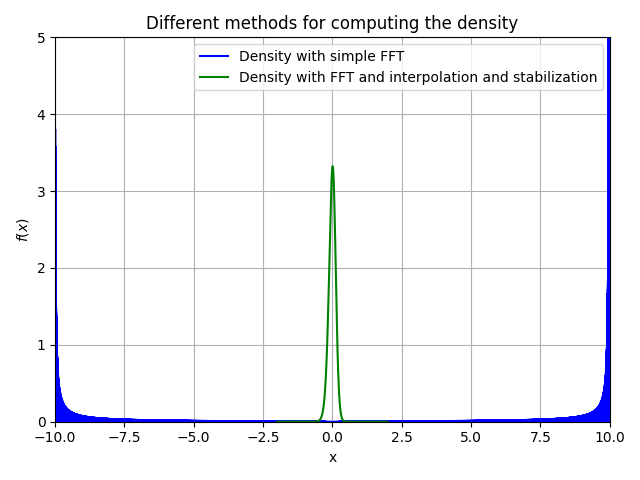
\includegraphics[width=0.8\textwidth]{img/different_ifft_methods.png}
    \caption{Comparison of different methods for the inverse Fourier transformation of the characteristic function of the Heston model ($\mu=0$, $\kappa=3$, $\theta=0.19$, $\sigma=0.4$, $\rho=-0.7$, $\tau=\frac{1}{12}$). Grid points: $N=2^{15}$}
    \label{fig:ifft_comparison}
\end{figure}

\subsection{Simulating the Heston Model}

- Heston Model is a model with continuous time, for simulation we need to discretize the time. Small timesteps require a lot of computational power, large timesteps can lead to zero or negative volatility if the so called Feller condition is not satisfied (Albrecher et al 2007). The Feller condition is satisfied if $2\kappa\theta > \sigma^2$ but Eraker et al (2003) show, that for S&P 500 index options the Feller condition is not satisfied. There are many more studies that show this result for other markets and assets (e.g. Chang et al 2021, Hu & Liu 2022).
- Intuitivster Weg der Zeit-Diskretisierung: Euler–Maruyama Diskretisierung:
\begin{align}
    X_{t+\Delta} &= X_t - \frac{1}{2}v_t\Delta + \sqrt{v_t}\sqrt{\Delta}Z_{X,t} \notag \\
    v_{t+\Delta} &= v_t + \kappa(\theta - v_t)\Delta + \sigma\sqrt{v_t}\sqrt{\Delta}Z_{v,t} \notag
\end{align}
wobei $Z\sim\mathcal{N}(0,1)$, $\Delta = T/n$, $T$ die gesamte Zeit und $n$ die Anzahl der Schritte ist. Die Korrelation zwischen $Z_{X,t}$ und $Z_{v,t}$ kann man wie folgt simulieren (Andersen 2008): %TODO: andere Quelle finden, nicht immer nur Andersen oder Ostap
\begin{align}
    Z_{v,t} &= \Phi^{-1}(U_1) \notag \\
    Z_{X,t} &= \rho Z_{v,t} + \sqrt{1-\rho^2}\Phi^{-1}(U_2) \notag
\end{align}
wobei $U_1$ und $U_2$ unabhängige Zufallsvariablen sind, die gleichverteilt sind auf $[0,1]$ und $\Phi^{-1}$ die inverse Verteilungsfunktion der Standardnormalverteilung ist.
- Bei dieser Diskretisierung sieht man auch gut das Problem der möglichen Negativität der Volatilität (Okhrin et al 2022):
\begin{align}
    \mathbb{P}(v_{t+\Delta}<0 \mid v_t>0) &= \mathbb{P}\left(Z_{v,t} < \frac{-v_t-\kappa(\theta-v_t)\Delta}{\sigma\sqrt{v_t}\sqrt{\Delta}}\right) \notag \\
    &= \Phi\left(Z_{v,t} < \frac{-v_t-\kappa(\theta-v_t)\Delta}{\sigma\sqrt{v_t}\sqrt{\Delta}}\right) \notag \\
    &> 0 \notag
\end{align}
wobei $\Phi$ die Verteilungsfunktion der Standardnormalverteilung ist. Es gibt verschiedene Methoden, um dieses Problem zu lösen, z.B. die Absorption (replace $v_t$ mit $v_t^+ = \max{0, v_t}$) oder Reflection Method (replace $v_t$ mit $\vert v_t\vert$). Alle diese Methoden ändern aber den unterliegenden Prozess, daher stimmen z.B. die Momente der Volatilität nicht mehr mit den theoretischen Momenten überein (Okhrin et al 2022, Tsoskounoglou 2024). 
- In der Studie von Okhrin et al (2022) Andersen's QE scheme performs best in terms of speed and accuracy. Andersen (2008) approximates the noncentral chi-square distribution in \eqref{eq:heston_model_variance_transition} with a mixture of distributions, a Dirac distribution and a noncentral Gaussian distribution. Für ausreichend große Werte von $v_t$ gilt
\begin{align}
    \label{eq:qe_normal}
    v_{t+\Delta} = a(b+Z_v)^2
\end{align}
mit $Z_v\sim\mathcal{N}(0,1)$. Für andere Werte von $v_t$ gilt
\begin{align}
    \label{eq:qe_dirac}
    v_{t+\Delta} &= \Psi^{-1}(U_v, p, \beta) \\
    \Psi^{-1}(u,p,\beta) &= \begin{cases}
        0 & 0\le u\le p \\
        \beta^{-1}\ln\left(\frac{1-p}{1-u}\right) & p<u\le 1
    \end{cases} \notag
\end{align}
Die Parameter $a$, $b$, $p$ und $\beta$ werden über moment-matching geschätzt, vom dem einen zum anderen Schema kann man wechseln, wenn der Wert $\psi$ über einer Schelle $\psi_c$ liegt. Dann nutzt man \eqref{eq:qe_dirac}, sonst \eqref{eq:qe_normal}. Der Wert $\psi$ ist der Quotient aus $s^2$ und $m^2$, wobei $m$ der Erwartungswert von $v_{t+\Delta}$ und $s^2$ die Varianz von $v_{t+\Delta}$ ist.
- Für den Preisprozess schlägt Andersen (2008) folgendes Schema vor:
\begin{align}
    \ln(S_{t+\Delta}) &= \ln(S_t) + K_0 + K_1v_t + K_2v_{t+\Delta} + \sqrt{K_3v_t + K_4v_{t+\Delta}}\cdot Z \notag \\
    K_0 &= -\frac{\rho\kappa\theta}{\sigma}\Delta \notag \\
    K_1 &= \xi_1\Delta\left(\frac{\kappa\rho}{\sigma} - \frac{1}{2}\right)-\frac{\rho}{\sigma} \notag \\
    K_2 &= \xi_2\Delta\left(\frac{\kappa\rho}{\sigma}-\frac{1}{2}\right)+\frac{\rho}{\sigma} \notag \\
    K_3 &= \xi_1\Delta(1-\rho^2) \notag \\
    K_4 &= \xi_2\Delta(1-\rho^2) \notag
\end{align}
wobei $Z$ standardnormalverteilt ist und $\xi_1$ und $\xi_2$ gewisse Konstanten sind, im Paper wird $\xi_1=\xi_2=0.5$ vorgeschlagen.
\chapter{Expansion Methods}
\label{sec:expansion_methods}

Expansion methods are series approximations of a probability density function. In general, these approximations are not true densities, as they can take negative values for certain parameter choices. However, for some parameter sets, they do define valid probability densities. In the following sections, we will explore the conditions under which expansion methods yield proper densities and how to transform a parameter set that does not correspond to a valid density into one that does.

\section{Gram-Charlier Expansion}
The Gram-Charlier expansion was introduced by Gram (\citeyear{gramUeberEntwickelungReeller1883}) and Charlier (\citeyear{charlierContributionsMathematicalTheory1914}). There are two types of expansions: Gram-Charlier A and Gram-Charlier B, which are defined as
\begin{align}
    f_{GC,A} &\approx f(x) + \sum_{k=3}^n a_k f^{(k)}(x) \notag \\
    f_{GC,B} &\approx \psi(x)\sum_{m=0}^n b_mg_m(x) \notag
\end{align}
Although these expansions can be applied to any density function $f$ and $\psi$, for Gram-Charlier Type A, the density $f$ is typically the standard normal distribution
\begin{align}
    f(x) = \frac{1}{\sqrt{2\pi}}\exp\left(-\frac{x^2}{2}\right) \notag
\end{align}
and for Gram-Charlier Type B, $\psi$ corresponds to the probability mass function of the Poisson distribution (\cite{mitropolskiiGramCharlierSeries2020}):
\begin{align}
    \psi(x) = \frac{\lambda^x}{x!}\exp(-\lambda) \notag
\end{align}
The term $f^{(k)}$ represents the $k$-th derivative of the density function $f$. There exist polynomials $H_k$ that satisfy
\begin{align}
    f^{(k)}(x) = (-1)^k f(x)H_k(x) \notag
\end{align}
These polynomials, known as Hermite polynomials, were studied by Laplace (\citeyear{laplaceMemoireIntegralesDefinies1811,laplaceTheorieAnalytiqueProbabilites1812}), Chebyshev (\citeyear{chebyshevDeveloppementFonctionsSeule1860}), and Hermite (\citeyear{hermiteNouveauDeveloppementSerie1864}). They have the following properties (\cite{abramowitzHandbookMathematicalFunctions1968}, p. 771ff):
\begin{align}
    H_{n+1} &= x\cdot H_n(x) - H'_n(x) \notag \\
    H'_n(x) &= n\cdot H_{n-1}(x) \notag \\
\end{align}
Using these recurrence relations, the first few Hermite polynomials can be computed as
\begin{align}
    H_{n+1}(x) &= x\cdot H_n(x) - nH_{n-1}(x) \notag \\
    H_0(x) &= 1 \notag \\
    H_1(x) &= x \notag \\
    H_2(x) &= x^2 - 1 \notag \\
    H_3(x) &= x^3-3x \notag \\
    H_4(x) &= x^4-6x^2+3 \notag \\
    H_5(x) &= x^5-10x^3+15x \notag \\
    H_6(x) &= x^6-15x^4+45x^2-15 \notag
\end{align}
The coefficients $a_k$ in the expansion can be expressed in terms of the moments $r_k$ of the density $f$. This leads to the first terms of the Gram-Charlier A expansion:
\begin{align}
    \label{eq:gc_a_expansion_kappa}
    f(x)_{GC,A} \approx &\, \frac{1}{\sqrt{2\pi}\sigma}\exp\left(-\frac{(x-\mu)^2}{2\sigma^2}\right) \notag\\[1ex]
    &\, \times \left[1 + \frac{\kappa_3}{6\sigma^3}H_3\left(\frac{x-\mu}{\sigma}\right)
    + \frac{\kappa_4}{24\sigma^4}H_4\left(\frac{x-\mu}{\sigma}\right)\right]
\end{align}
where $\mu$, $\sigma^2$, $\kappa_3$, and $\kappa_4$ represent the first four cumulants of the target distribution. Based on Equations \eqref{eq:cumulants_1} and \eqref{eq:cumulants_2}, $\mu$ and $\sigma^2$ correspond to the first two cumulants $\kappa_1$ and $\kappa_2$.

The first terms of the Gram-Charlier B expansion are given by
\begin{align}
    f(x)_{GC,B} \approx &\; \frac{\lambda^x}{x!}\exp(-\lambda) \notag\\[1ex]
    &\; \times \Biggl( 1 
       + \frac{\mu_2 - \lambda}{\lambda^2}\Bigl[\frac{x^{[2]}}{2} - \lambda x^{[1]} + \frac{\lambda^2}{2}\Bigr] \notag\\[1ex]
    &\quad + \frac{\mu_3 - 3\mu_2 + 2\lambda}{\lambda^3}\Bigl[\frac{x^{[3]}}{6} - \frac{\lambda}{2}x^{[2]} + \frac{\lambda^2}{2}x^{[1]} - \frac{\lambda^3}{6}\Bigr] \Biggr) \notag
\end{align}    
where $\mu_i$ are the central moments of the target distribution, and $x^{[i]} = x(x-1)\dots (x-i+1)$ (\cite{mitropolskiiGramCharlierSeries2020}). However, since Gram-Charlier Type B only allows discrete values for $x$, it cannot be applied to continuous distributions. Therefore, we focus exclusively on Gram-Charlier Type A in this work.

\section{Gram-Charlier Expansion with Positivity Constraints}

The Gram-Charlier expansion can take negative values, which is not permissible for a probability density function. Jondeau \& Rockinger (\citeyear{jondeauGramCharlierDensities2001}) analyzed the conditions under which the expansion remains a valid density. By using Equations \eqref{eq:cumulants_3} and \eqref{eq:cumulants_4}, Equation \eqref{eq:gc_a_expansion_kappa} can be rewritten in terms of the skewness $\gamma_1$ and excess kurtosis $\gamma_2^*$, defining $z = \frac{x-\mu}{\sigma}$:
\begin{align}
    \label{eq:gc_a_expansion_s_ek}
    f(x)_{GC,A} \approx \frac{1}{\sqrt{2\pi}}\exp\left(-\frac{z^2}{2}\right) \left[1 + \frac{\gamma_1}{6}H_3(z) + \frac{\gamma_2^*}{24}H_4(z)\right]
\end{align}
To determine when the Gram-Charlier expansion remains a valid density, the following condition must hold:
\begin{align}
    1 + \frac{\gamma_1}{6}He_3(z) + \frac{\gamma_2^*}{24}He_4(z) &= 0 \notag \\
    \frac{\gamma_1}{6}He_3(z) &= -1 - \frac{\gamma_2^*}{24}He_4(z) \notag \\
    \gamma_1\cdot He_3(z) &= -6 - \frac{\gamma_2^*}{4}He_4(z) \notag \\
    \gamma_1 &= -\frac{6}{He_3(z)} - \frac{He_4(z)}{4\cdot He_3(z)}\gamma_2^* \notag \\
    \gamma_1 &= \frac{z^4-6z^2+3}{12z-4z^3}\cdot \gamma_2^* + \frac{24}{12z-4z^3} \notag
\end{align}
This leads to a boundary condition for the skewness and excess kurtosis, illustrated in Figures \ref{fig:gram_charlier_boundary_lines_20_vs_1000} and \ref{fig:gram_charlier_boundary}.

Using a bisection algorithm and a logistic mapping, Jondeau \& Rockinger (\citeyear{jondeauGramCharlierDensities2001}) construct a piecewise linear boundary, ensuring that any unconstrained pair $(\tilde{\gamma_1}, \tilde{\gamma_2^*}) \in \mathbb{R}^2$ is mapped to a constrained pair within the positivity region $\mathcal{D}$. Finding a closed-form expression for the boundary is computationally difficult; even with 24 hours on a high-performance computer using Python's SymPy library, no explicit solution was found.

A comparison between constrained and unconstrained parameters for four distributions—standard normal, lognormal, $t$-distribution, and non-central $t$-distribution—is presented in Table \ref{table:distributions_theoretical_moments} and Figures \ref{fig:gc_expansion} and \ref{fig:gc_positivity_expansion}. The results highlight the necessity of positivity constraints, which, however, distort the expansion, particularly for cases where no constraints were originally required (e.g., the standard normal distribution). The logistic mapping shifts the excess kurtosis from 0 to 2, mapping the unconstrained pair $(\tilde{\gamma_1}, \tilde{\gamma_2^*}) = (0,0)$ to the constrained pair $(\gamma_1, \gamma_2^*) = (0,2)$.

\begin{figure}[h]
    \centering
    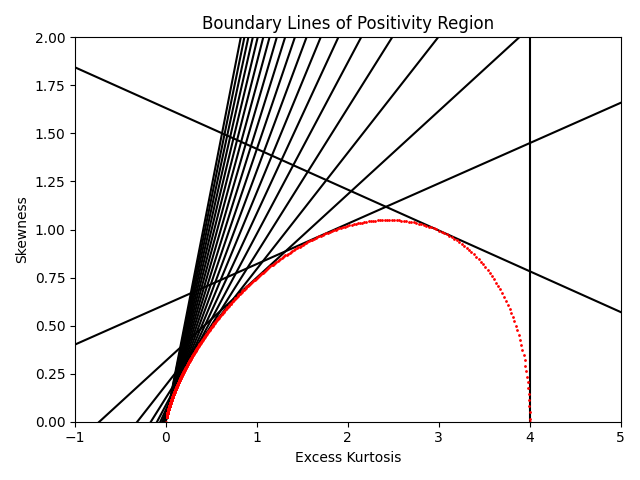
\includegraphics[width=0.4\textwidth]{img/gc_positivity_boundary_lines_20.png}
    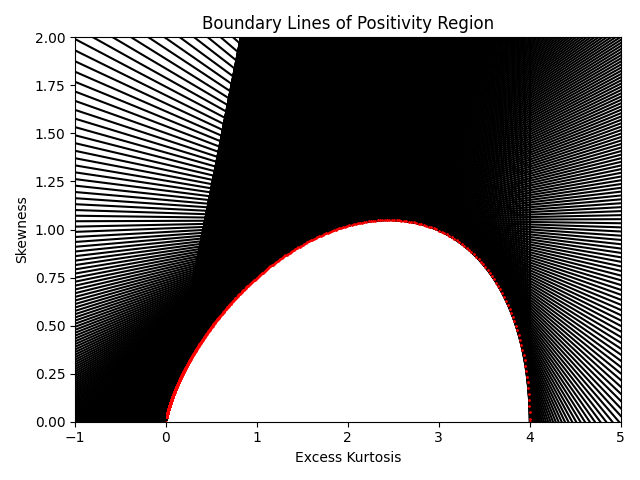
\includegraphics[width=0.4\textwidth]{img/gc_positivity_boundary_lines_1000.png}
    \caption{Boundary lines of the positivity region of the Gram-Charlier Expansion. The left image shows 20 lines, the right image shows 1000 lines. The red dots are the boundary points. The boundary is symmetric to the x-axis.}
    \label{fig:gram_charlier_boundary_lines_20_vs_1000}
\end{figure}

\begin{figure}[h]
    \centering
    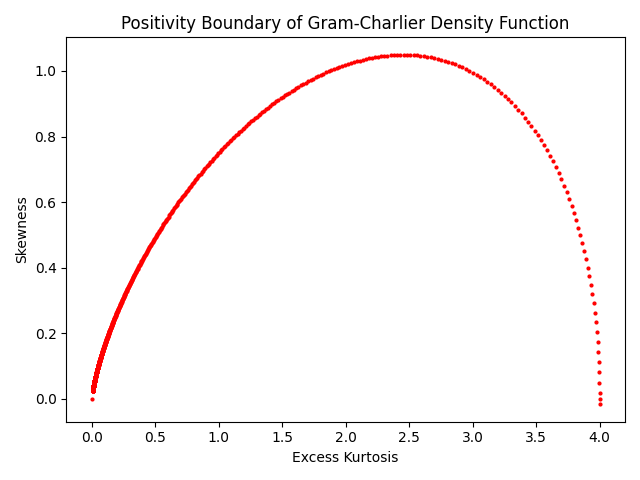
\includegraphics[width=0.8\textwidth]{img/gc_positivity_boundary.png}
    \caption{Approximation (1000 steps) of the positivity boundary of the Gram-Charlier Expansion. For simplicity, only the part above the x-axis is shown. The boundary is symmetric to the x-axis.}
    \label{fig:gram_charlier_boundary}
\end{figure}

\begin{table}[h]
    \centering
    \begin{tabular}{l|l|l|l|l|l|l|l}
        Distribution & $\mu$ & $\sigma^2$ & $\kappa_3$ & $\gamma_1$ & $\kappa_4$ & $\gamma_2^*$ \\
        \hline
        $\mathcal{N}(\mu=0,\sigma1)$ & 0 & 1 & 0 & 0 & 0 & 0 \\
        $\mathcal{L}(\mu=0, \sigma=0.5)$ & 1.1331 & 0.3647 & 0.3855 & 1.7502 & 0.7845 & 5.8984 \\
        $\mathcal{T}(\nu=5)$ & 0 & 1.6667 & 0 & 0 & 16.6667 & 6 \\
        $\mathcal{NCT}(\nu=5, \mu=0.5)$ & 0.5947 & 1.7297 & 1.5357 & 0.6751 & 21.5969 & 7.2189
    \end{tabular}
    \caption{Distribution parameters and theoretical moments and cumulants. $\mathcal{N}$ stands for the Normal distribution, $\mathcal{L}$ for the Lognormal distribution, $\mathcal{T}$ for the Student's $t$-distribution, and $\mathcal{NCT}$ for the Non-Central $t$-distribution.}
    \label{table:distributions_theoretical_moments}
\end{table}

\begin{figure}[h]
    \centering
    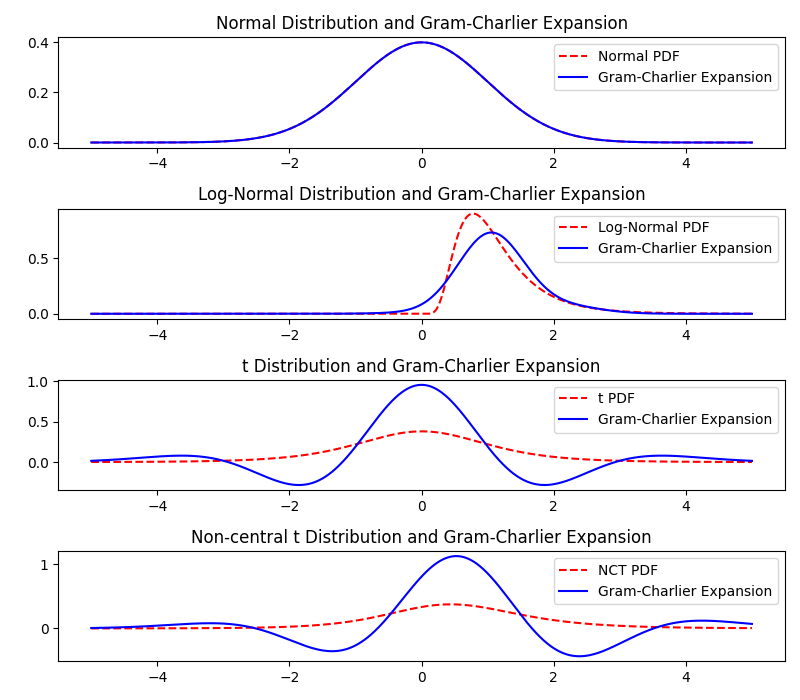
\includegraphics[width=0.8\textwidth]{img/gc_expansion.png}
    \caption{Gram-Charlier Expansion of different distributions}
    \label{fig:gc_expansion}
\end{figure}

\begin{figure}[h]
    \centering
    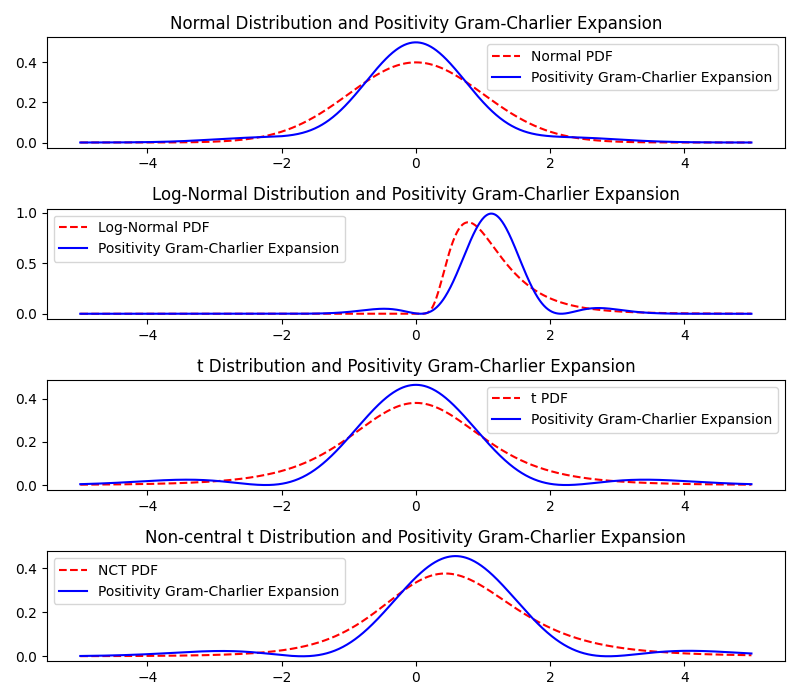
\includegraphics[width=0.8\textwidth]{img/gc_positivity_expansion.png}
    \caption{Gram-Charlier Expansion with positivity constraints of different distributions}
    \label{fig:gc_positivity_expansion}
\end{figure}

\section{Edgeworth Expansion}

The Gram-Charlier expansion is not an asymptotic expansion, as it does not allow for a well-defined approximation error. The Edgeworth expansion, however, is an asymptotic expansion (\cite{cramerMathematicalMethodsStatistics1999}, Section 17.6) and is therefore preferred. An asymptotic expansion consists of a series of functions $f_n$ that, after a finite number of terms, approximate a function at a specific point $\xi$ (often infinite) as $x$ approaches $\xi$:
\begin{align}
    f_{n+1}(x) = o(f_n(x)) \quad x\to\xi \notag
\end{align}

Originally introduced by Edgeworth (\citeyear{edgeworthRepresentationStatisticalFrequency1907}), who suggested computing the approximation up to the sixth term to mitigate the issues associated with asymptotic expansions. A formal representation of the first terms can be found in Brenn \& Anfinsen (\citeyear{brennRevisitGramCharlierEdgeworth2017}).
\begin{align}
    f(x)_{EW} \approx &\; \frac{1}{\sqrt{2\pi}\sigma}\exp\left(-\frac{(x-\mu)^2}{2\sigma^2}\right) \notag\\[1ex]
    &\; \times \Biggl[ 1 
        + \frac{\kappa_3}{6\sigma^3}H_3\left(\frac{x-\mu}{\sigma}\right) + \frac{\kappa_4}{24\sigma^4}H_4\left(\frac{x-\mu}{\sigma}\right) \notag\\[1ex]
    &\quad + \frac{\kappa_5}{120\sigma^5}H_5\left(\frac{x-\mu}{\sigma}\right) + \frac{\kappa_6 + 10\kappa_3^2}{720\sigma^6}H_6\left(\frac{x-\mu}{\sigma}\right)
    \Biggr] \notag
\end{align}
    
Since this work only considers the first four cumulants, the expression simplifies to:
\begin{align}
    f(x)_{EW} \approx {} & \frac{1}{\sqrt{2\pi}\sigma}\exp\left(-\frac{(x-\mu)^2}{2\sigma^2}\right)\notag\\[1ex]
    & \quad \times \Biggl[ 1 
       + \frac{\kappa_3}{6\sigma^3}H_3\left(\frac{x-\mu}{\sigma}\right) + \frac{\kappa_4}{24\sigma^4}H_4\left(\frac{x-\mu}{\sigma}\right) \notag\\[1ex]
    \label{eq:ew_expansion_short}
    & \quad \quad + \frac{\kappa_3^2}{72\sigma^6}H_6\left(\frac{x-\mu}{\sigma}\right)
    \Biggr]
\end{align}    

\section{Edgeworth Expansion with Positivity Constraints}

Following the approach of Jondeau \& Rockinger (\citeyear{jondeauGramCharlierDensities2001}) for the Gram-Charlier expansion, we determine the positivity boundary for the Edgeworth expansion by rewriting Equation \eqref{eq:ew_expansion_short} using $z = \frac{x-\mu}{\sigma}$:
\begin{align}
    \label{eq:ew_expansion_s_ek}
    f(x)_{EW} \approx \frac{1}{\sqrt{2\pi}}\exp\left(-\frac{z^2}{2}\right) \left[1 + \frac{\gamma_1}{6}H_3(z) + \frac{\gamma_2^*}{24}H_4(z) + \frac{\gamma_1^2}{72}He_6(z)\right]
\end{align}
To ensure the expansion remains a valid density, we solve for skewness $\gamma_1$ in the equation:
\begin{align}
    0 &= 1+\frac{\gamma_1}{6}He_3(z) + \frac{\gamma_2^*}{24}He_4(z) + \frac{\gamma_1^2}{72}He_6(z) \\
    \gamma_1 &= \pm\sqrt{-\frac{72}{He_6(z)} - 3\gamma_2^*\frac{He_4(z)}{He_6(z)} + 36\frac{He_3(z)^2}{He_6(z)^2}} - 6\frac{He_3(z)}{He_6(z)} \notag
\end{align}
This equation is valid as long as $H_6(z) \neq 0$, which occurs at six points:
\begin{align}
    z_{1/2} &= \pm \sqrt{5-\frac{5^{2/3}\left(1+i\sqrt{3}\right)}{\sqrt[3]{2\left(2+i\sqrt{6}\right)}} - \frac{\left(1-i\sqrt{3}\right)\sqrt[3]{5\left(2+i\sqrt{6}\right)}}{2^{2/3}}} = \pm 0.6167 \notag\\
    z_{3/4} &= \pm \sqrt{5-\frac{5^{2/3}\left(1-i\sqrt{3}\right)}{\sqrt[3]{2\left(2+i\sqrt{6}\right)}} - \frac{\left(1+i\sqrt{3}\right)\sqrt[3]{5\left(2+i\sqrt{6}\right)}}{2^{2/3}}} = \pm 1.8892 \notag \\
    z_{5/6} &= \pm \sqrt{5+\frac{10^{2/3}}{\sqrt[3]{2+i\sqrt{6}}} + \sqrt[3]{10\left(2+i\sqrt{6}\right)}} = \pm 3.3243 \notag
\end{align}

\begin{figure}[h]
    \centering
    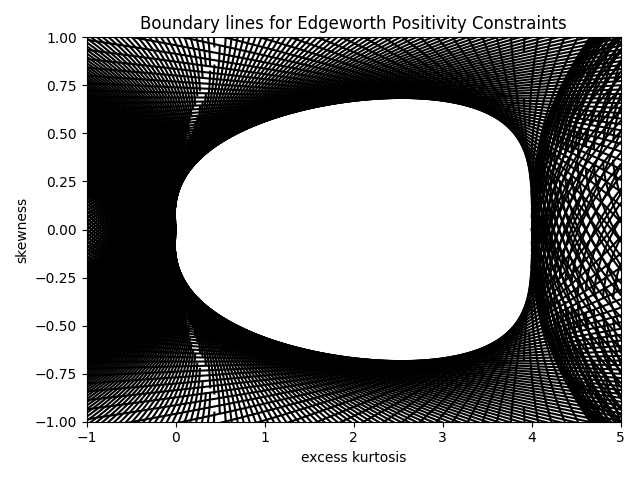
\includegraphics[width=0.8\textwidth]{img/edgeworth_positivity_boundary_lines.png}
    \caption{Boundary Lines for Edgeworth Expansion}
    \label{fig:ew_boundary_lines}
\end{figure}
\begin{figure}[h]
    \centering
    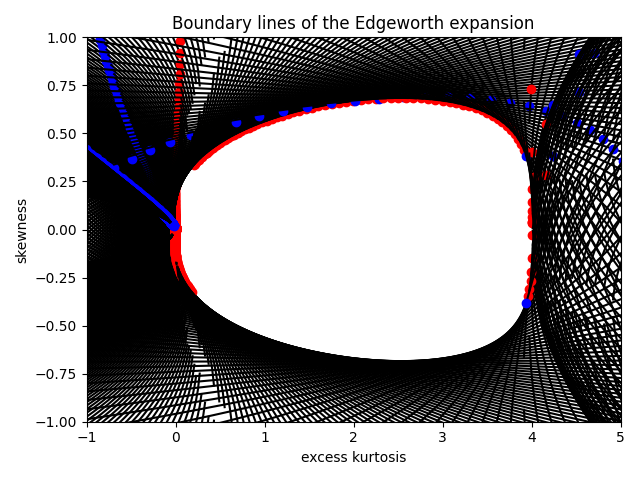
\includegraphics[width=0.8\textwidth]{img/edgeworth_positivity_boundary_intersections_1.png}
    \caption{Intersections of Boundary Lines for Edgeworth Expansion, red is first intersection, blue is second intersection}
    \label{fig:ew_boundary_intersections_1}
\end{figure}
\begin{figure}[h]
    \centering
    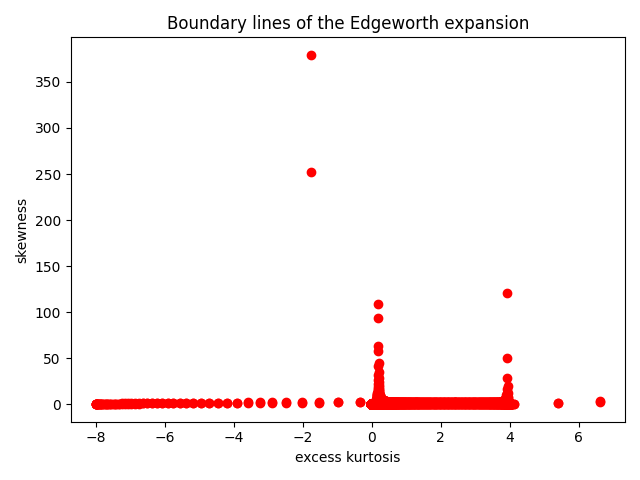
\includegraphics[width=0.8\textwidth]{img/edgeworth_positivity_boundary_intersections_3.png}
    \caption{Intersections of Boundary Lines for Edgeworth Expansion (zoomed out), upper half}
    \label{fig:ew_boundary_intersections_3}
\end{figure}
\begin{figure}[h]
    \centering
    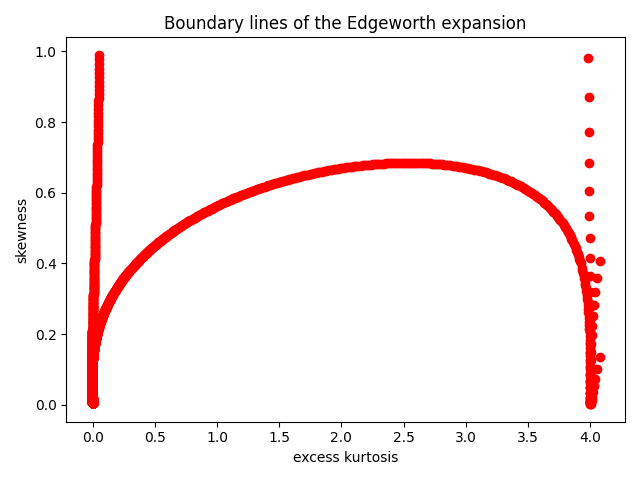
\includegraphics[width=0.8\textwidth]{img/edgeworth_positivity_boundary_intersections_4.png}
    \caption{Intersections of Boundary Lines for Edgeworth Expansion (zoomed in), upper half}
    \label{fig:ew_boundary_intersections_4}
\end{figure}
\begin{figure}[h]
    \centering
    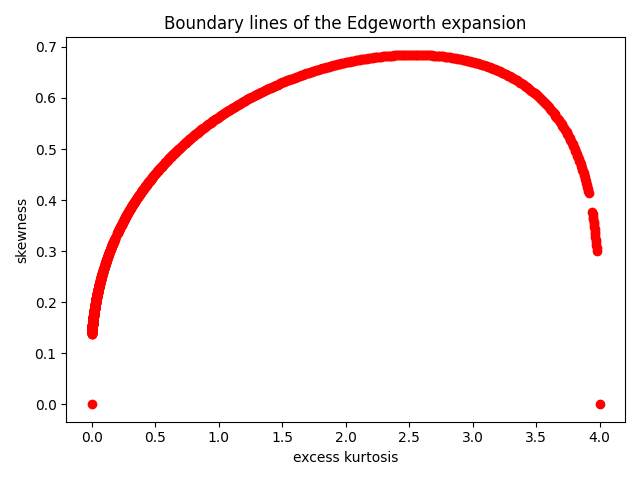
\includegraphics[width=0.8\textwidth]{img/edgeworth_positivity_boundary_intersections_7.png}
    \caption{Final Boundary Points for Edgeworth Expansion, upper half}
    \label{fig:ew_boundary_intersections_7}
\end{figure}

The positivity boundary for the Edgeworth expansion is determined by plotting the lines $\gamma_1(\gamma_2^*, z)$ for many values of $z$, skipping over the six singularities. Figure \ref{fig:ew_boundary_lines} shows that the positivity region for the Edgeworth expansion is smaller than for the Gram-Charlier expansion. For $\gamma_1 = 0$, the excess kurtosis is constrained between 0 and 4, which matches the boundary of the Gram-Charlier expansion since both expansions are identical when skewness is zero.

As with the Gram-Charlier expansion, the positivity boundary is given by the envelope of the lines $\gamma_1(\gamma_2^*, z)$. We obtain this by computing the intersections of pairs of parabolic equations. The equations are too long to be displayed here, you can find them in the corresponding GitHub repository\footnote{\url{https://github.com/henrydatei/heston-moments-pdf}}. These intersections are shown in Figures \ref{fig:ew_boundary_intersections_1} to \ref{fig:ew_boundary_intersections_7}.

Since each $\gamma_1(\gamma_2^*, z)$ equation is a parabola, the positivity region can be computed by:
\begin{enumerate}
    \item Ignoring the second intersection for each $z$-value (since the first intersection defines the boundary). The boundary is symmetric around the $x$-axis, so we only compute the upper half and mirror it afterward.
    \item Filtering out non-relevant points: Figure \ref{fig:ew_boundary_intersections_3} shows many extraneous intersection points. Based on previous results, we restrict the solutions to $\gamma_2^* \in (-0.1,4.1)$ and $\vert \gamma_1\vert \in [0,1)$. (see Figure \ref{fig:ew_boundary_intersections_4})
    \item Removing points from non-relevant boundary lines: The lower-boundary artifacts arise from $z$-values smaller than the third singularity; these are removed. The upper-boundary artifacts come from $\vert z \vert$ around 1.8 and 1.67, and are filtered out by removing all $z$ in the ranges $(1.8-0.035, 1.8+0.035)$ and $(1.67-0.015,1.67+0.015)$.
    \item Computational accuracy is a concern since some points lie slightly outside the expected range (e.g., one point is at $(\gamma_2^*, \gamma_1) = (4.01, 0.222)$). Testing this point in the Edgeworth expansion shows that it does not satisfy the positivity condition:
    \begin{align}
        1 + \frac{0.222}{6}He_3(z) + \frac{4.01}{24}He_4(z) + \frac{0.222^2}{72}He_6(z)<0 \notag
    \end{align}
    gives a solution: $-1.84611<z<-1.75826$. This might be due to Python's float datatype which maps to IEEE-754 double precision with 64 bits where 52 bits are used for the fraction which equals about 16 decimal digits (\cite{pythonfoundation15FloatingPointArithmetic,leonardo.zAnswerHowCan2013}). To be conservative, we remove any intersection with $\gamma_2^* \notin [0,4]$.
    \item Adding the points $(0,0)$ and $(4,0)$ completes the positivity region. A linear interpolation between the closest computed boundary points results in the final positivity boundary (see Figure \ref{fig:ew_boundary_intersections_7}).
\end{enumerate}

\begin{figure}[h]
    \centering
    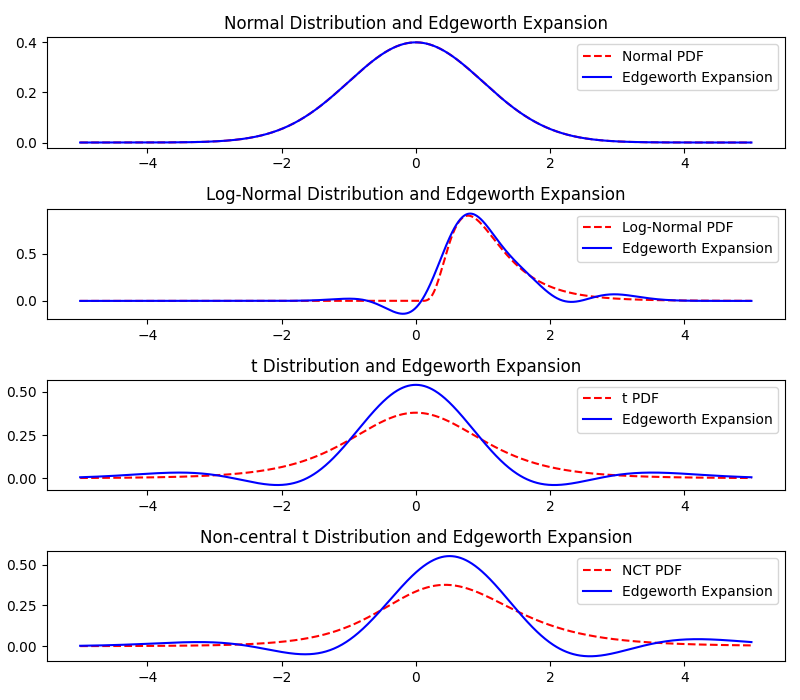
\includegraphics[width=0.8\textwidth]{img/ew_expansion.png}
    \caption{Edgeworth Expansion of different distributions}
    \label{fig:ew_expansion}
\end{figure}

\begin{figure}[h]
    \centering
    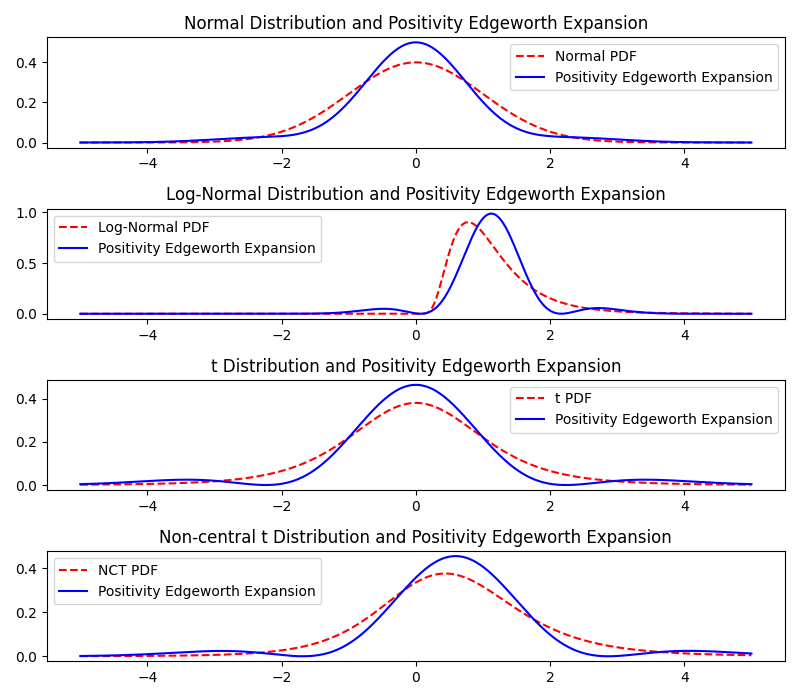
\includegraphics[width=0.8\textwidth]{img/ew_positivity_expansion.png}
    \caption{Edgeworth Expansion with positivity constraints of different distributions}
    \label{fig:ew_positivity_expansion}
\end{figure}

As with the Gram-Charlier expansion, we compare the constrained and unconstrained parameters for four distributions: standard normal, lognormal, $t$-distribution, and non-central $t$-distribution (see Table \ref{table:distributions_theoretical_moments}). The results, shown in Figures \ref{fig:ew_expansion} and \ref{fig:ew_positivity_expansion}, lead to the same conclusion as in the Gram-Charlier case: Positivity constraints are necessary, but they also distort the expansion and even when constraints are not needed (e.g., for the standard normal distribution), applying the positivity constraints artificially increases excess kurtosis from 0 to 2.
\chapter{Implementation of the Simulation Study}
\label{sec:methodical_approach}

\section{Carrying out the Simulation}
All the methods introduced in the previous chapters were implemented in Python. To analyze their behavior, we conducted a simulation of $n = 1$ paths of the Heston model using the Quadratic Exponential (QE) scheme by Andersen (\citeyear{andersenEfficientSimulationHeston2007}). Since the results are averaged over time, simulating multiple paths was deemed unnecessary. The simulation was based on interday 5-minute price data, with 79 observations per trading day, 22 trading days per month, 12 months per year, and a total simulation period of 15 years ($T = 15$), leading to 312,840 prices per path. A burn-in period of three years was applied to eliminate biases stemming from the initial price $S_0 = 100$ and initial volatility $v_0$.

The simulation covered a broad parameter space inspired by the estimates of Eraker (\citeyear{erakerStockPricesVolatility2004}). Specifically, $v_0$ ranged from 0.01 to 0.5 in steps of 0.05, $\kappa$ from 0.01 to 1 in steps of 0.1, $\theta$ from 0.01 to 1 in steps of 0.05, and $\sigma$ from 0.01 to 1 in steps of 0.05. The drift parameter $\mu$ took only two values, 0 and 0.05, while the correlation $\rho$ varied from -0.9 to 0.9 in steps of 0.1. In total, the simulation encompassed 1,440,000 parameter combinations.

Preliminary tests revealed that the QE scheme occasionally produces numerical errors, particularly when the Feller condition is strongly violated. A closer inspection of these cases showed that the issue manifests as an excessive number of price values clustering at the same level. To systematically detect these errors, the frequency of the most common price value was recorded for the first simulated path of each scenario. In simulations without errors, this frequency remained in the single-digit range, whereas in faulty simulations, it surged into the hundreds or thousands, indicating numerical instability.

For each simulated path, we computed the first four realized moments, skewness, and kurtosis following Neuberger \& Payne (\citeyear{neubergerSkewnessStockMarket2021}), as well as the first four cumulants based on Fukasawa \& Matsushita (\citeyear{fukasawaRealizedCumulantsMartingales2021}). Since this process is computationally intensive, requiring approximately 100 seconds per simulation on a 1.8 GHz Dual-Core Intel Core i5, parallelization was employed to improve efficiency. To manage large-scale data output, each computing core stored its results in a separate CSV file, minimizing write conflicts. The collected data was then merged into a central database for further analysis.

Additionally, for each simulation, we computed the theoretical mean, variance, skewness, and kurtosis of the returns based on the closed-form expressions derived in Okhrin et al. (\citeyear{okhrinDistributionalPropertiesContinuous2023}). Since these quantities depend only on the model parameters, they could be computed efficiently using basic arithmetic operations, allowing their calculation to be performed directly within the database.

\section{Calculating Results}
For each simulation, the Gram-Charlier expansion, the Gram-Charlier expansion with positivity constraints, the Edgeworth expansion, the Edgeworth expansion with positivity constraints, the Cornish-Fisher expansion, and the Saddlepoint approximation are computed. Each expansion method is applied to both the first four realized moments and the first four cumulants.

To evaluate the accuracy of these expansions, the theoretical density is derived from the characteristic function and compared to the densities obtained from the expansions using the Kolmogorov-Smirnov test (\cite{kolmogorovSullaDeterminazioneEmpirica1993}), the Cramér-von Mises test (\cite{vonmisesWahrscheinlichkeitStatistikUnd1928, cramerCompositionElementaryErrors1928, andersonDistributionTwoSampleCramervon1962}), and the Anderson-Darling test (\cite{andersonTestGoodnessFit1954}). While the Kolmogorov-Smirnov test measures the overall fit between two distributions, the Cramér-von Mises test and the Anderson-Darling test place greater emphasis on the tails of the distribution. This is particularly relevant for financial markets, where heavy tails arise due to crises and market crashes. The Cramér-von Mises test is less sensitive to the tails than the Anderson-Darling test, providing a balanced assessment of goodness-of-fit.

Since these tests require samples drawn from the cumulative distribution function (CDF), a numerical CDF is constructed from the density by performing cumulative summation and normalizing all values so that the last element equals 1.

Additionally, to further analyze the tails of the distributions, the Hill estimator is used to estimate the tail index $\alpha$ (\cite{hillSimpleGeneralApproach1975}). The tail index is a shape parameter that characterizes the power-law behavior of a distribution, where larger values of $\alpha$ indicate thinner tails (\cite{fischlerAnswerDefinitionTailindex2017, danielssonTailIndexEstimation2016}).

As previously noted in the discussion on the Heston model, the formula in Equation \eqref{eq:heston_model_characteristic_function_C} can lead to overflow errors, as Python's floating-point arithmetic is limited to values in the range $10^{-308}$ to $10^{308}$. To address this, the reformulated expression in Equation \eqref{eq:heston_model_characteristic_function_C_2} is used for computations.
\chapter{Results}
\label{sec:results}

\section{Findings from the Simulations}
- Wie in Vorversuchen schon bemerkt: QE-Schema produziert numerische Fehler, die sich darin zeigen, dass Preise mehrfach in der Simulation vorkommen. Bei korrekter Simulation ist der häufigste Preis im ersten Pfad im einstelligen Bereich, bei Fehlern im Hunderter- oder Tausenderbereich.
- Abbildung \ref{fig:max_number_of_same_prices_distribution} zeigt die Verteilung, man sieht einen Peak bei 1, was darauf hindeutet, dass die meisten Simulationen korrekt sind. Man sieht aber auch, dass es einige Simulationen gibt, wo der selbe Preis bis zu 250000 mal vorkommt, hier kam es zu numerischen Fehlern. Bei diesen Simulationen stellt man fest, dass, wenn es das erste Mal zu numerischen Fehlern kommt, der Rest der Zeitreihe den selben Preis hat. Bei Simulationen mit 250000 gleichen Preises kam es also sehr früh in der Zeitreihe zu einem numerischen Fehler.

\begin{figure}
    \centering
    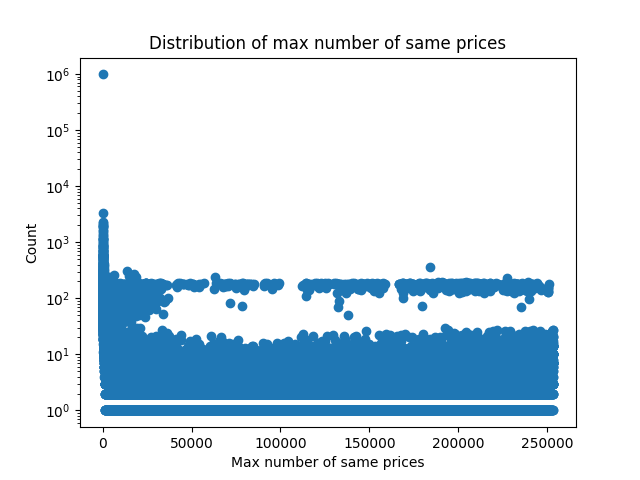
\includegraphics[width=0.8\textwidth]{img/max_number_of_same_prices_distribution.png}
    \caption{Distribution of the maximum number of the same prices in the first path of the simulation}
    \label{fig:max_number_of_same_prices_distribution}
\end{figure}

- Für die weitere Untersuchung sollen solche Simulationen ausgeschlossen werden, da sie nicht korrekt sind. Da es durchaus möglich ist, dass es auch bei korrekter Simulation zu gleichen Preisen kommt, wird ein Schwellwert gesucht, sodass möglichst viele korrekte Simulationen in der Untersuchung bleiben. Abbildung \ref{fig:max_number_of_same_prices_cumulative_percentage} zeigt für verschiedene Schwellwerte (die maximale Anzahl an gleichen Preisen) den kumulativen Anteil der Simulationen, die diesen Schwellwert nicht überschreiten. Wählt man den Schwellwert 1, also nur Simulationen, bei denen nie ein Preis mehrfach vorkommt, verbleiben bleiben 68.40\% der Simulation. Je höher man den Schwellwert setzt, desto weniger Simulationen fallen weg, aber unter Umständen verbleiben auch Simulationen, die numerische Fehler enthalten. Das betrifft aber nur sehr wenige Simulationen, der Anteil an inkludierten Simulationen steigt fast gar nicht. Für die späteren Untersuchungen werden also alle Simulationen entfernt, bei denen der selbe Preis mehr als einmal vorkommt.

\begin{figure}
    \centering
    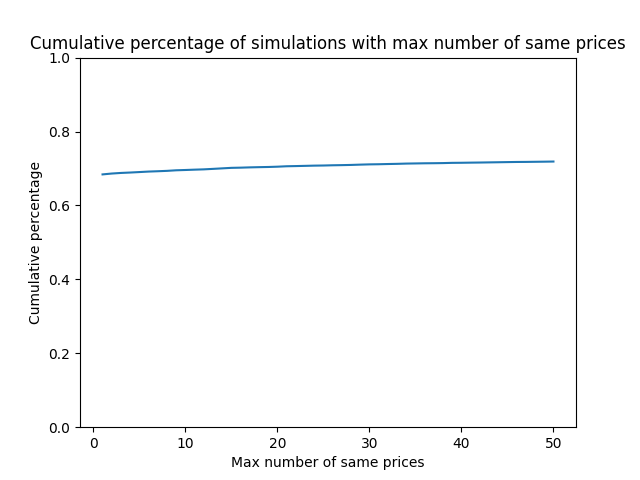
\includegraphics[width=0.8\textwidth]{img/max_number_of_same_prices_cumulative_percentage.png}
    \caption{Cumulative percentage of simulations that do not exceed the maximum number of same prices}
    \label{fig:max_number_of_same_prices_cumulative_percentage}
\end{figure}

\begin{figure}
    \centering
    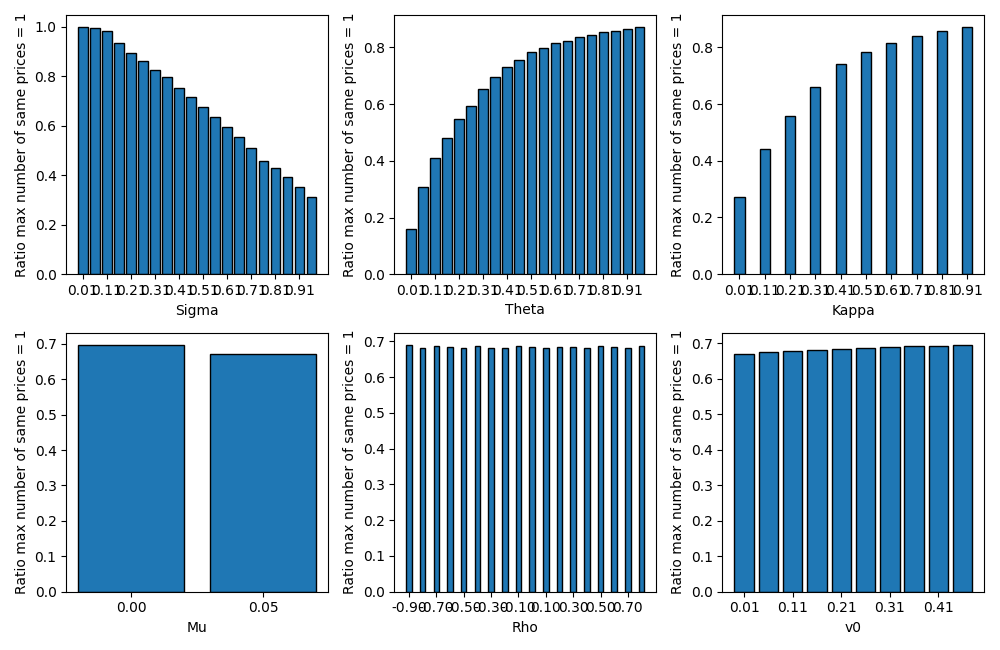
\includegraphics[width=0.8\textwidth]{img/max_number_of_same_prices_ratio_parameters.png}
    \caption{Ratio of simulations that do not exceed the maximum number of same prices in relation to the parameters of the Heston model}
    \label{fig:max_number_of_same_prices_ratio_parameters}
\end{figure}

\begin{figure}
    \centering
    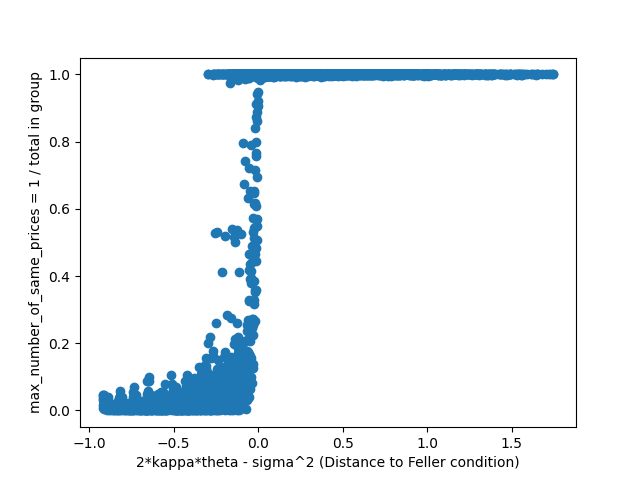
\includegraphics[width=0.8\textwidth]{img/max_number_of_same_prices_ratio_feller_diff.png}
    \caption{Ratio of simulations that do not exceed the maximum number of same prices in relation to the value $D$}
    \label{fig:max_number_of_same_prices_ratio_D}
\end{figure}

- Untersuchung, woher diese Fehler kommen: Dazu bestimmen des Anteils der Simulationen, die korrekt in Abhängigkeit eines jeden einzelnen Parameters des Heston-Modells (siehe Abbildung \ref{fig:max_number_of_same_prices_ratio_parameters}). Man erkennt, dass mit zunehmendem $\sigma$ die Fehler zunehmen, während mit zunehmendem $\theta$ und $\kappa$ die Fehler abnehmen. Die Parameter $\mu$, $\rho$ und $v_0$ haben keinen Einfluss auf die Fehlerhäufigkeit. Das legt nahe, dass die Fehler mit der Feller condition zusammenhängen. Deshalb untersuche ich nun die Fehlerhäufigkeit und den Wert $D = 2\kappa\theta - \sigma^2$. Ist dieser Wert positiv, so ist die Feller condition erfüllt, je negativer er ist, desto weniger erfüllt ist die Feller condition. Abbildung \ref{fig:max_number_of_same_prices_ratio_D} zeigt, dass, sobald die Feller condition nicht mehr erfüllt ist, die Fehlerhäufigkeit stark zunimmt. Wenn die Feller condition erfüllt ist, so sind 99.90\% der Simulationen korrekt, ist die Feller condition nicht erfüllt, so sind es nur 25.48\%. Insgesamt erfüllen 57.80\% der Simulationen die Feller condition.
- Im Folgenden werden einige Expansionsmethoden weiter untersucht, gestartet wird mit der Gram-Charlier-Expansion, da sie die einfachste Methode ist.

\section{Investigating the Results for the Gram-Charlier-Expansion}

\subsection{Comparing with the Kolmogorov-Smirnov-Test}

\begin{figure}
    \centering
    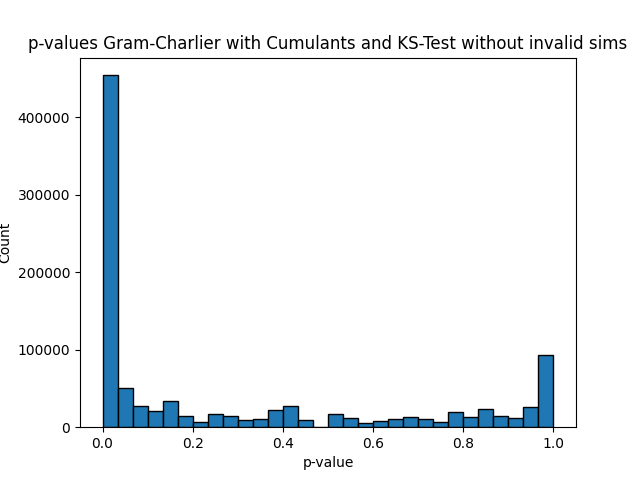
\includegraphics[width=0.8\textwidth]{img/GC_cum_KS_p_value_histogram.png}
    \caption{Distribution of p values of the Kolmogorov-Smirnov-Test for the Gram-Charlier Expansion with Cumulants vs the theoretical density without invalid simulations}
    \label{fig:GC_cum_KS_p_value_histogram}
\end{figure}

- In Abbildung \ref{fig:GC_cum_KS_p_value_histogram} sieht man die Verteilung der p values des Kolmogorov-Smirnov-Tests für die Gram-Charlier Expansion mit Kumulanten im Vergleich zur theoretischen Dichte. Dabei wurden alle Simulationen entfernt, bei denen der selbe Preis mehr als einmal vorkommt. Ein p Wert von über 5\% bedeutet, dass es keine signifikanten Unterschiede zwischen den beiden Verteilungen gibt, die Gram-Charlier Expansion auf Basis von Kumulanten approximiert die theoretische Dichte also gut genug. Man sieht, dass dies für einige Parameterkombinationen nicht der Fall ist; insgesamt für 52.48\% der Simulationen. Für restliche Expansionsmethoden siehe Tabelle \ref{tab:KS_p_value_percentage}.

\begin{table}[h]
    \centering
    \begin{tabular}{l|c|c|c|c|c|c}
        & \textbf{Gram-Charlier} & \textbf{GC+} & \textbf{Edgeworth} & \textbf{EW+} & \textbf{Cornish-Fisher} & \textbf{Saddlepoint} \\
        \hline
        \textbf{Cumulants} & 52.48\% & 47.63\% & 52.14\% & 47.64\% & 35.85\% & 45.36\% \\
        \textbf{Moments} & 37.35\% & 21.24\% & 36.02\% & 23.27\% & 44.90\% & 40.92\%
    \end{tabular}
    \caption{Percentage of simulations where the p-value of the Kolmogorov-Smirnov-Test against the theoretical density is above 5\%. Invalid simulations are excluded. GC+ and EW+ stand for the Gram-Charlier Expansion with positivity constraint and the Edgeworth Expansion with positivity constraint, respectively.}
    \label{tab:KS_p_value_percentage}
\end{table}

- Wir untersuchen nun, ob es Zusammenhänge zwischen den Parametern des Heston-Modells und den p Werten des Kolmogorov-Smirnov-Tests gibt. Abbildung \ref{fig:pairplot_GC_cum_KS_muzero} zeigt einen Pairplot für alle Parameterkombinationen (außer $\mu$) und die p Werte des Kolmogorov-Smirnov-Tests für die Gram-Charlier Expansion
mit Kumulanten gegen die theoretische Dichte. Je heller die Region ist, desto höher ist der Anteil an p values über 5\% und damit desto öfter approximiert die Gram-Charlier Expansion mit Kumulanten die theoretische Dichte gut.
- Der Parameter $\mu$ wurde auf 0 gesetzt, da sämtliche Verfahren zur Schätzung der Momente und Kumulanten nur für Preisprozesse funktioniert, die Martingales sind. 
- Man sieht in den Farbverläufen, welche Parameter einen Einfluss zu haben scheinen, das trifft auf $\sigma$, $\kappa$ und $\theta$ zu. Der Parameter $\rho$ scheint eher keinen Einfluss haben, egal wie man diesen Parameter wählt und den anderen Parameter fixiert, die Farbe ändert sich nicht. Selbiges gilt für $v_0$. Man würde auch erwarten, dass $v_0$ keinen Einfluss hat, da $v_0$ die Startvolatilität ist und wir, um die unbedingten Momente und Kumulanten zu bestimmen, einen Burnin von 3 Jahren (bei 15 Jahren Simulationsdauer) verwenden. 
- Für den Parameter $\sigma$ sieht man, dass dieser so gering wie möglich sein sollte, während $\kappa$ so hoch wie möglich sein sollte. Die Wahl des Parameters $\theta$ scheint schwieriger zu sein, da es keine klare Tendenz gibt. Grundsätzlich scheint $\theta$ mit steigendem $\kappa$ auch größer gewählt werden, zum anderen sollte bei kleinem $\sigma$ auch ein kleines $\theta$ gewählt werden.
\begin{figure}
    \centering
    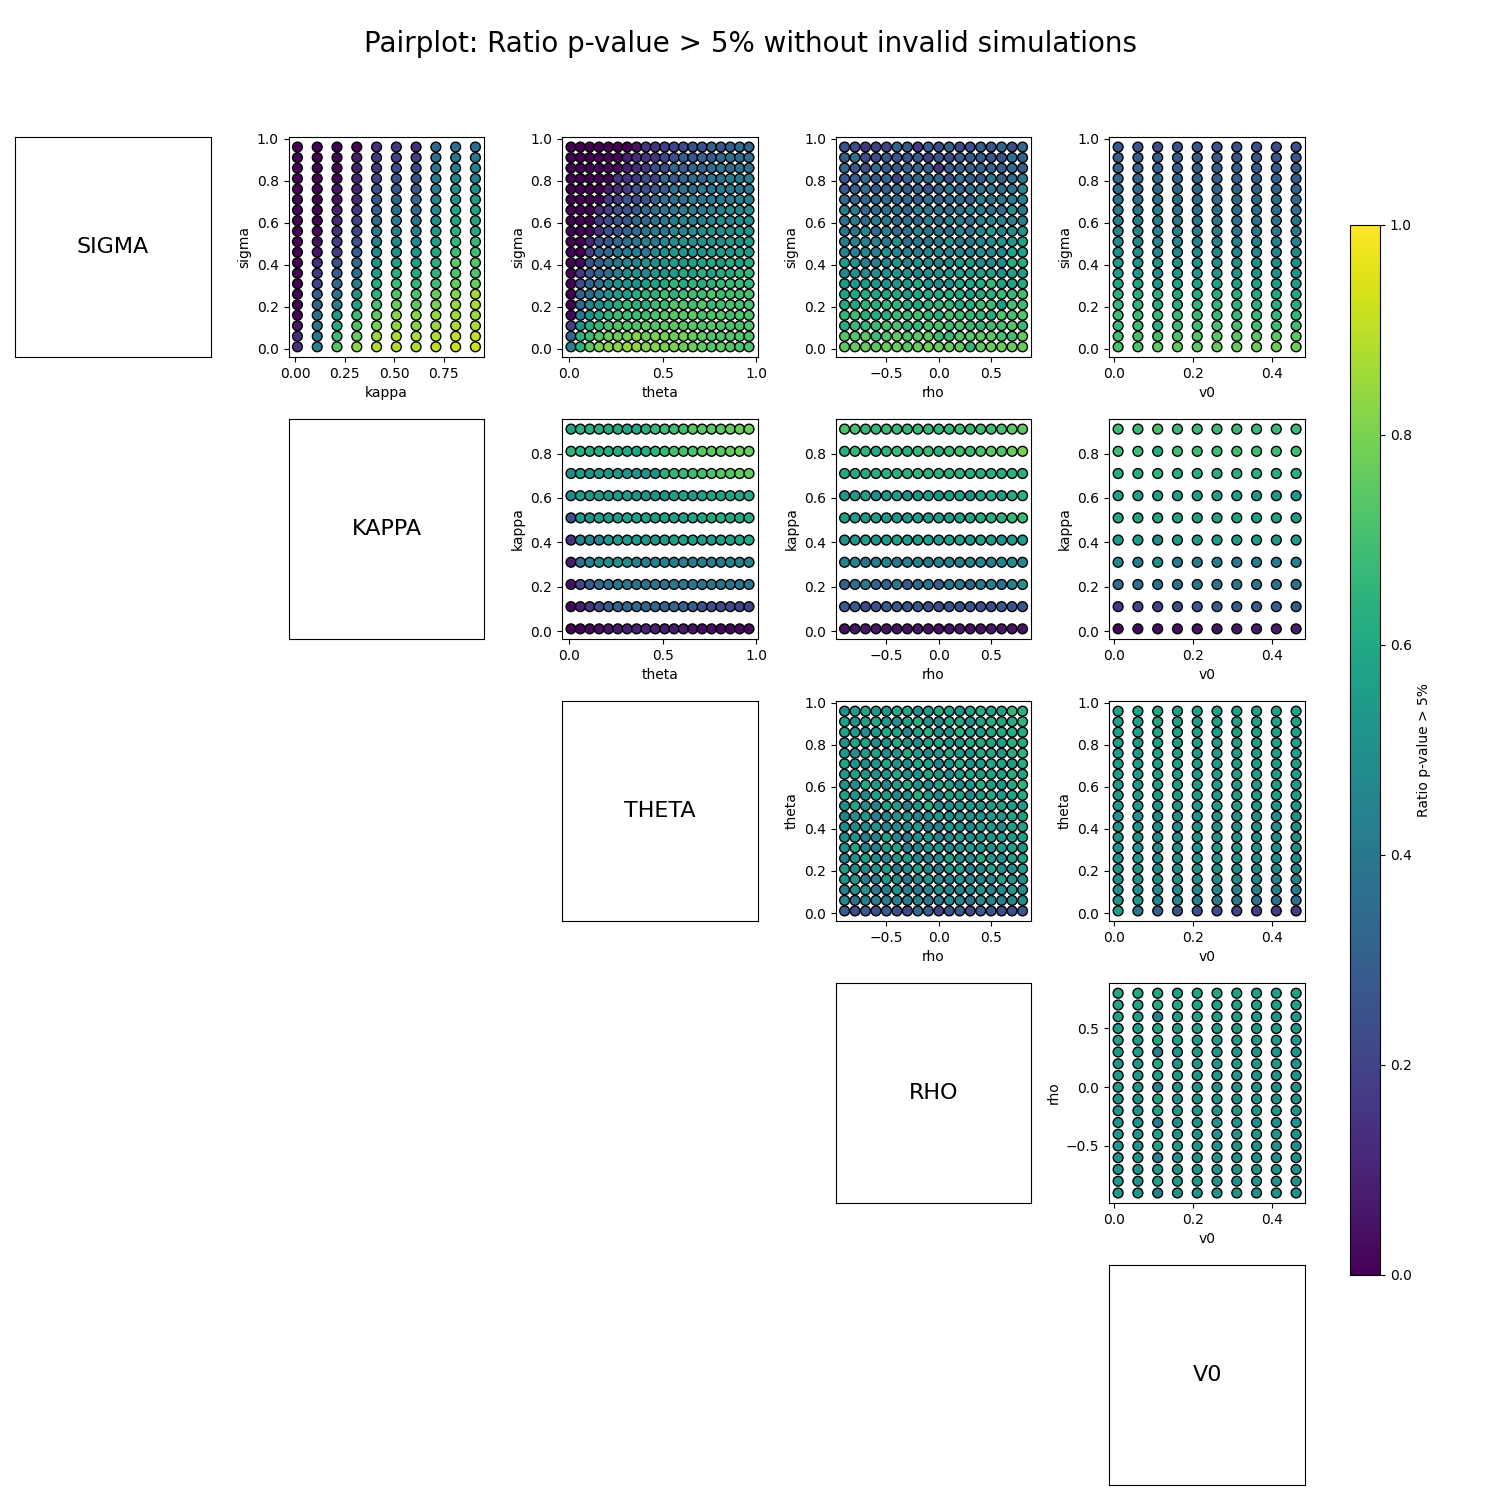
\includegraphics[width=0.8\textwidth]{img/pairplot_GC_cum_KS_muzero.png}
    \caption{Pairplot for each pair of parameters for the Heston Model and the percentage of p values of the Kolmogorov-Smirnov-Test for the Gram-Charlier Expansion with Cumulants vs the theoretical density above 5\%. Invalid simulations are excluded and $\mu=0$.}
    \label{fig:pairplot_GC_cum_KS_muzero}
\end{figure}

\begin{figure}
    \centering
    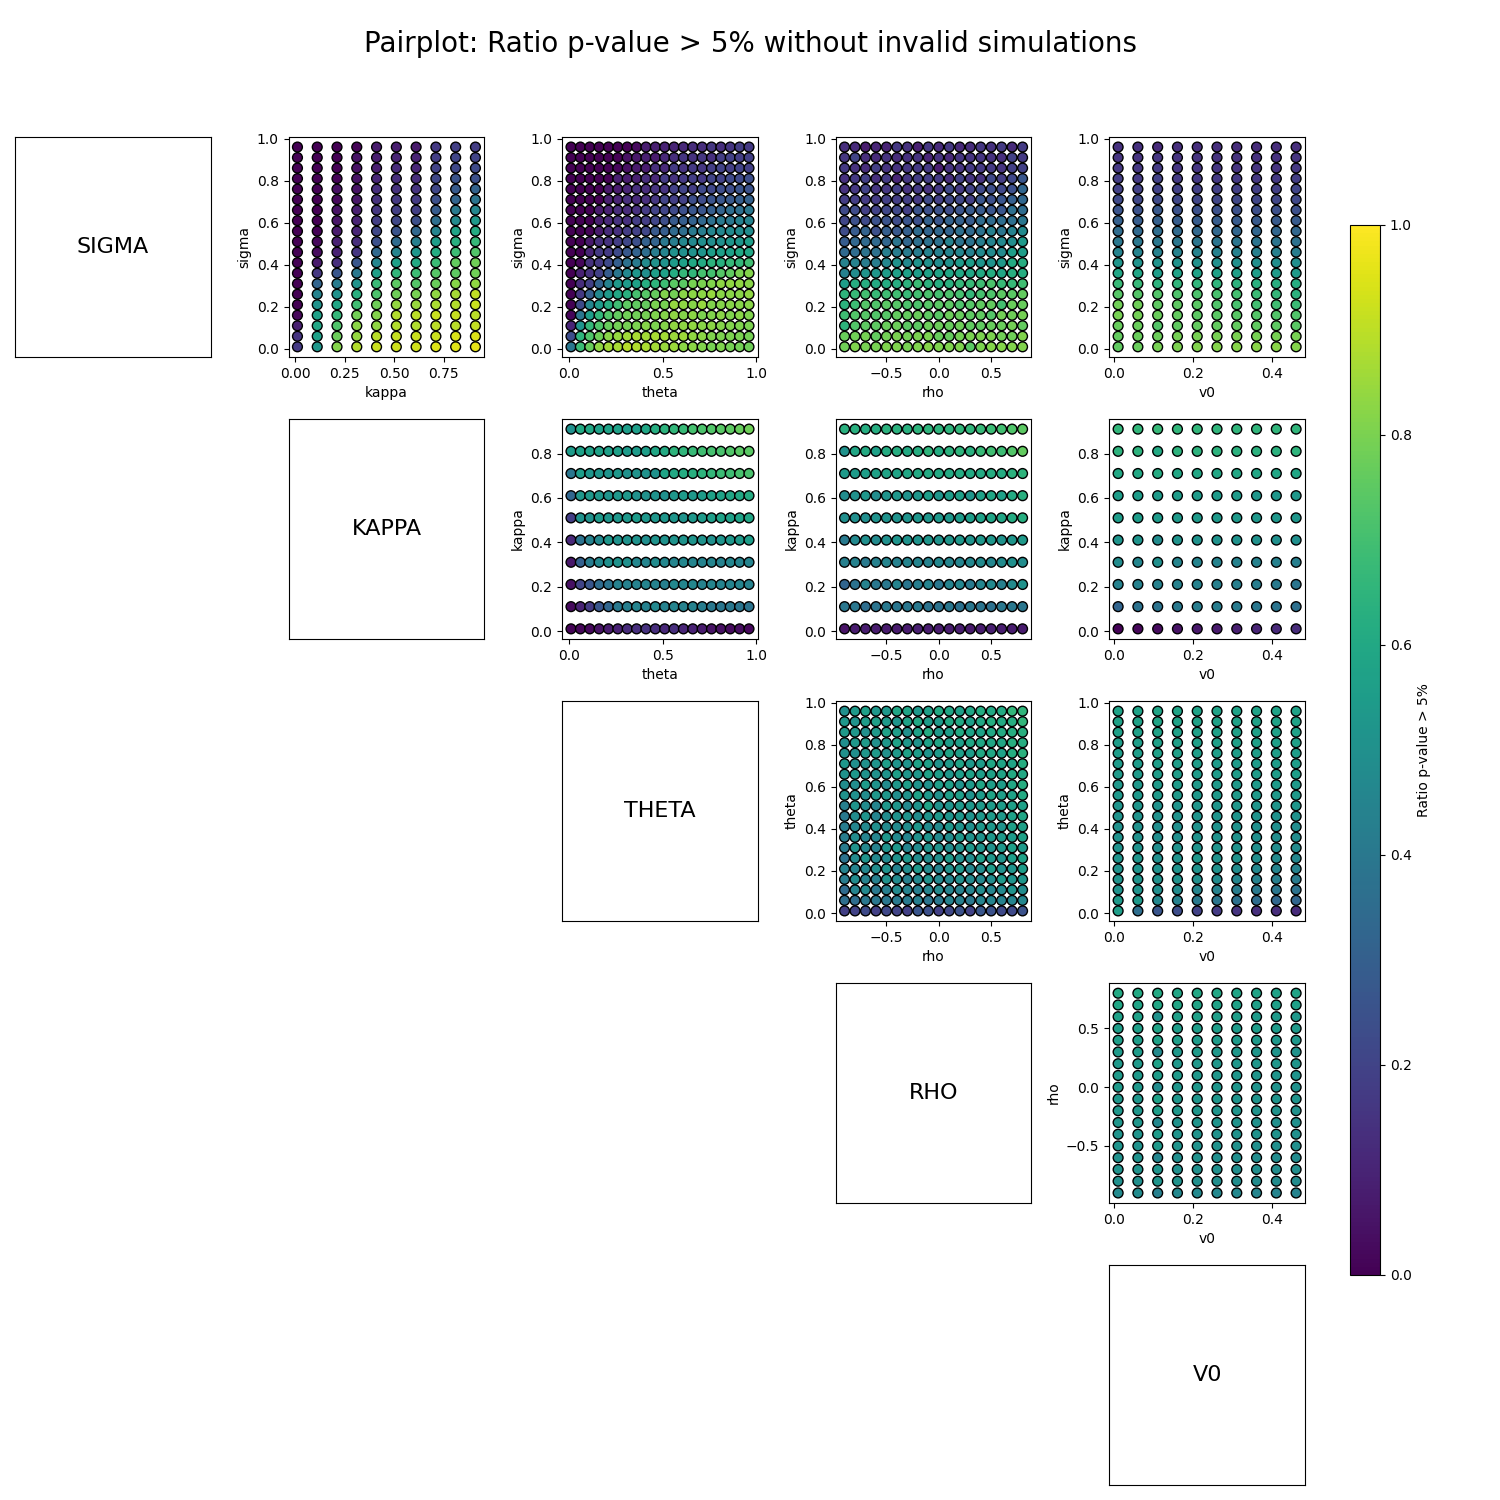
\includegraphics[width=0.8\textwidth]{img/pairplot_GC_cum_KS.png}
    \caption{Pairplot for each pair of parameters for the Heston Model and the percentage of p values of the Kolmogorov-Smirnov-Test for the Gram-Charlier Expansion with Cumulants vs the theoretical density above 5\%. Invalid simulations are excluded and $\mu=0.05$.}
    \label{fig:pairplot_GC_cum_KS_mu005}
\end{figure}

- Wir können schauen, wie sich der Pairplot Abbildung \ref{fig:pairplot_GC_cum_KS_muzero} ändert, wenn wir die Bedingung, dass der Preisprozess ein Martingale sein muss, verletzen. Dazu setzen wir $\mu=0.05$ und erhalten Abbildung \ref{fig:pairplot_GC_cum_KS_mu005}. Es fällt direkt auf, dass es weiße Stellen im Diagramm gibt. Das sind die Fälle, bei denen durch das Herausfiltern aller ungültigen Simulationen keine Simulationen mehr übrig bleiben. Das ist immer dann der Fall, wenn die Feller condition stark nicht erfüllt ist, also $2\kappa\theta - \sigma^2 <0$. Interessant ist, dass dieser Effekt nur bei $\mu=0.05$ so stark zum Tragen kommt, bei $mu=0$ fielen nicht so viele Simulationen weg.
- Der andere, sehr überraschende Punkt ist, dass es insgesamt mehr gelbe Punkte gibt, die Gram-Charlier-Expansion sich also -- für passend gewählte Parameter -- besser an die theoretische Dichte annähert, wenn der Preisprozess kein Martingale ist. Im Gegenzug gibt es aber auch mehr Parameterkombinationen (insbesondere $\sigma$, $\kappa$ und $\theta$), bei denen sich die Gram-Charlier-Expansion schlechter an die theoretische Dichte annähert.

\begin{figure}
    \centering
    \begin{subfigure}[b]{0.4\textwidth}
        \centering
        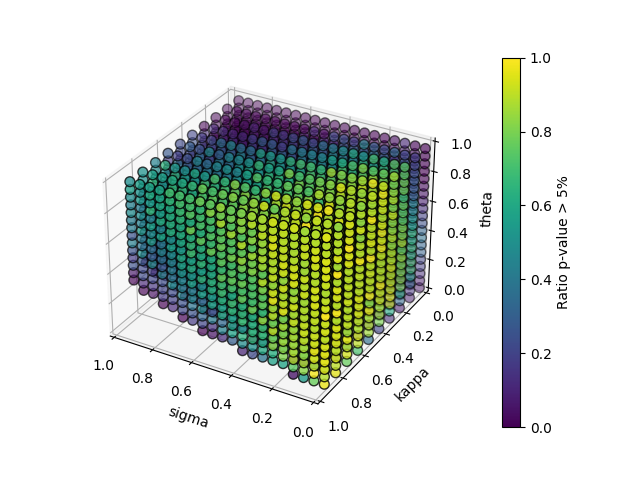
\includegraphics[width=\textwidth]{img/GC_cum_KS_3d_p_value_sigma_kappa_theta_muzero.png}
        \caption{$\mu=0$}
        \label{fig:GC_cum_KS_3d_p_value_sigma_kappa_theta_muzero}
    \end{subfigure}
    \hfill
    \begin{subfigure}[b]{0.4\textwidth}
        \centering
        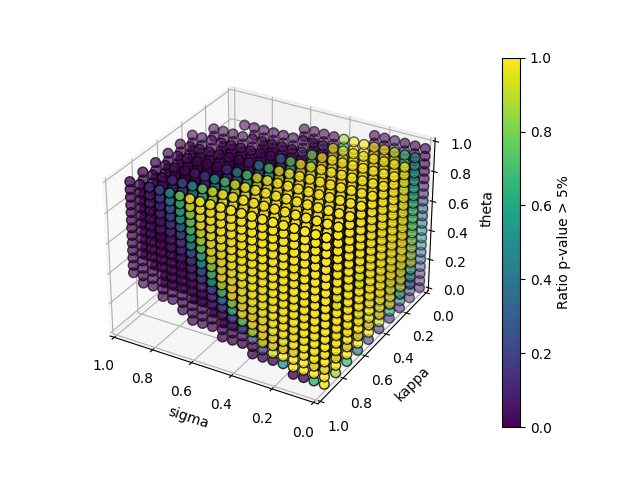
\includegraphics[width=\textwidth]{img/GC_cum_KS_3d_p_value_sigma_kappa_theta.png}
        \caption{$\mu=0.05$}
        \label{fig:GC_cum_KS_3d_p_value_sigma_kappa_theta}
    \end{subfigure}
    \caption{Percentage of simulations where the p-value of the Kolmogorov-Smirnov-Test against the theoretical density is above 5\%. Invalid simulations are excluded.}
    \label{fig:GC_cum_KS_3d}
\end{figure}

- In der detaillierteren Darstellung \ref{fig:GC_cum_KS_3d} sieht man besonders deutlich den Unterschied zwischen $mu=0$ (Abbildung \ref{fig:GC_cum_KS_3d_p_value_sigma_kappa_theta_muzero}) und $mu=0.05$ (Abbildung \ref{fig:GC_cum_KS_3d_p_value_sigma_kappa_theta}). Aus Gründen der Übersichtlichkeit wurde nicht noch eine Fläche eingezeichnet, ab wann die Feller condition erfüllt und nicht erfüllt ist, aber fast alle Punkte in Abbildung \ref{fig:GC_cum_KS_3d_p_value_sigma_kappa_theta} liegen innerhalb des Bereiches, in dem die Feller condition erfüllt ist, während es in Abbildung \ref{fig:GC_cum_KS_3d_p_value_sigma_kappa_theta_muzero} auch Punkte gibt, die außerhalb liegen. Es ist unklar, wie sich dieser Bereich charakterisieren lässt, die Feller condition bzw die Distanz $D$ reicht dafür nicht aus.

\subsection{Comparing the Tails with the Anderson-Darling-Test}

- Persönlich hätte ich vermutet, dass sich die Ergebnisse ändern, wenn man nun einen Test verwendet, der stärker auf die Ränder der Verteilung reagiert, wie den Anderson-Darling-Test. Aber man sieht, dass es praktisch keinen Unterschied zwischen den Abbildungen \ref{fig:pairplot_GC_cum_AD_muzero} + \ref{fig:pairplot_GC_cum_AD_mu005} und den Abbildungen \ref{fig:pairplot_GC_cum_KS_muzero} + \ref{fig:pairplot_GC_cum_KS_mu005} gibt.

\begin{figure}
    \centering
    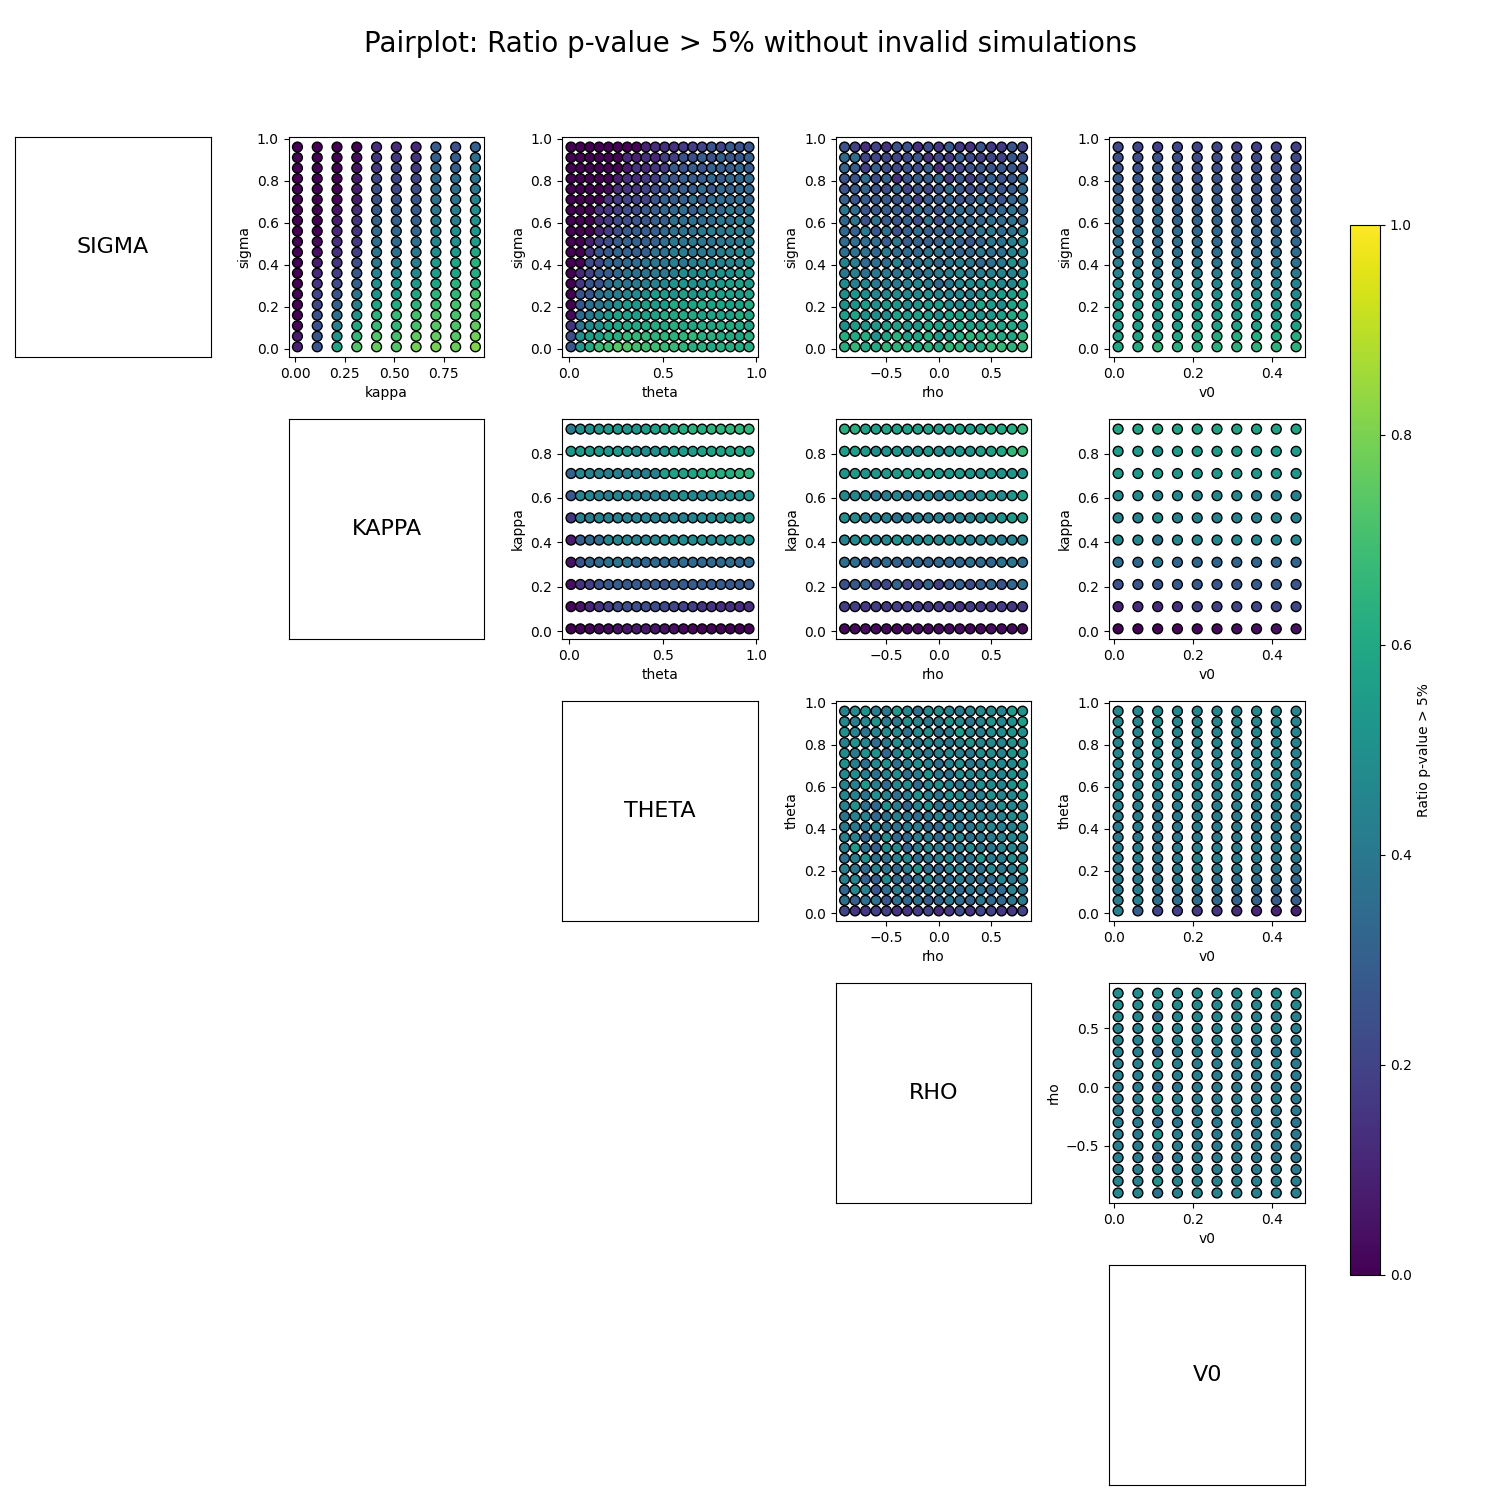
\includegraphics[width=0.8\textwidth]{img/pairplot_GC_cum_AD_muzero.png}
    \caption{Pairplot for each pair of parameters for the Heston Model and the percentage of p values of the Anderson-Darling-Test for the Gram-Charlier Expansion with Cumulants vs the theoretical density above 5\%. Invalid simulations are excluded and $\mu=0$.}
    \label{fig:pairplot_GC_cum_AD_muzero}
\end{figure}

\begin{figure}
    \centering
    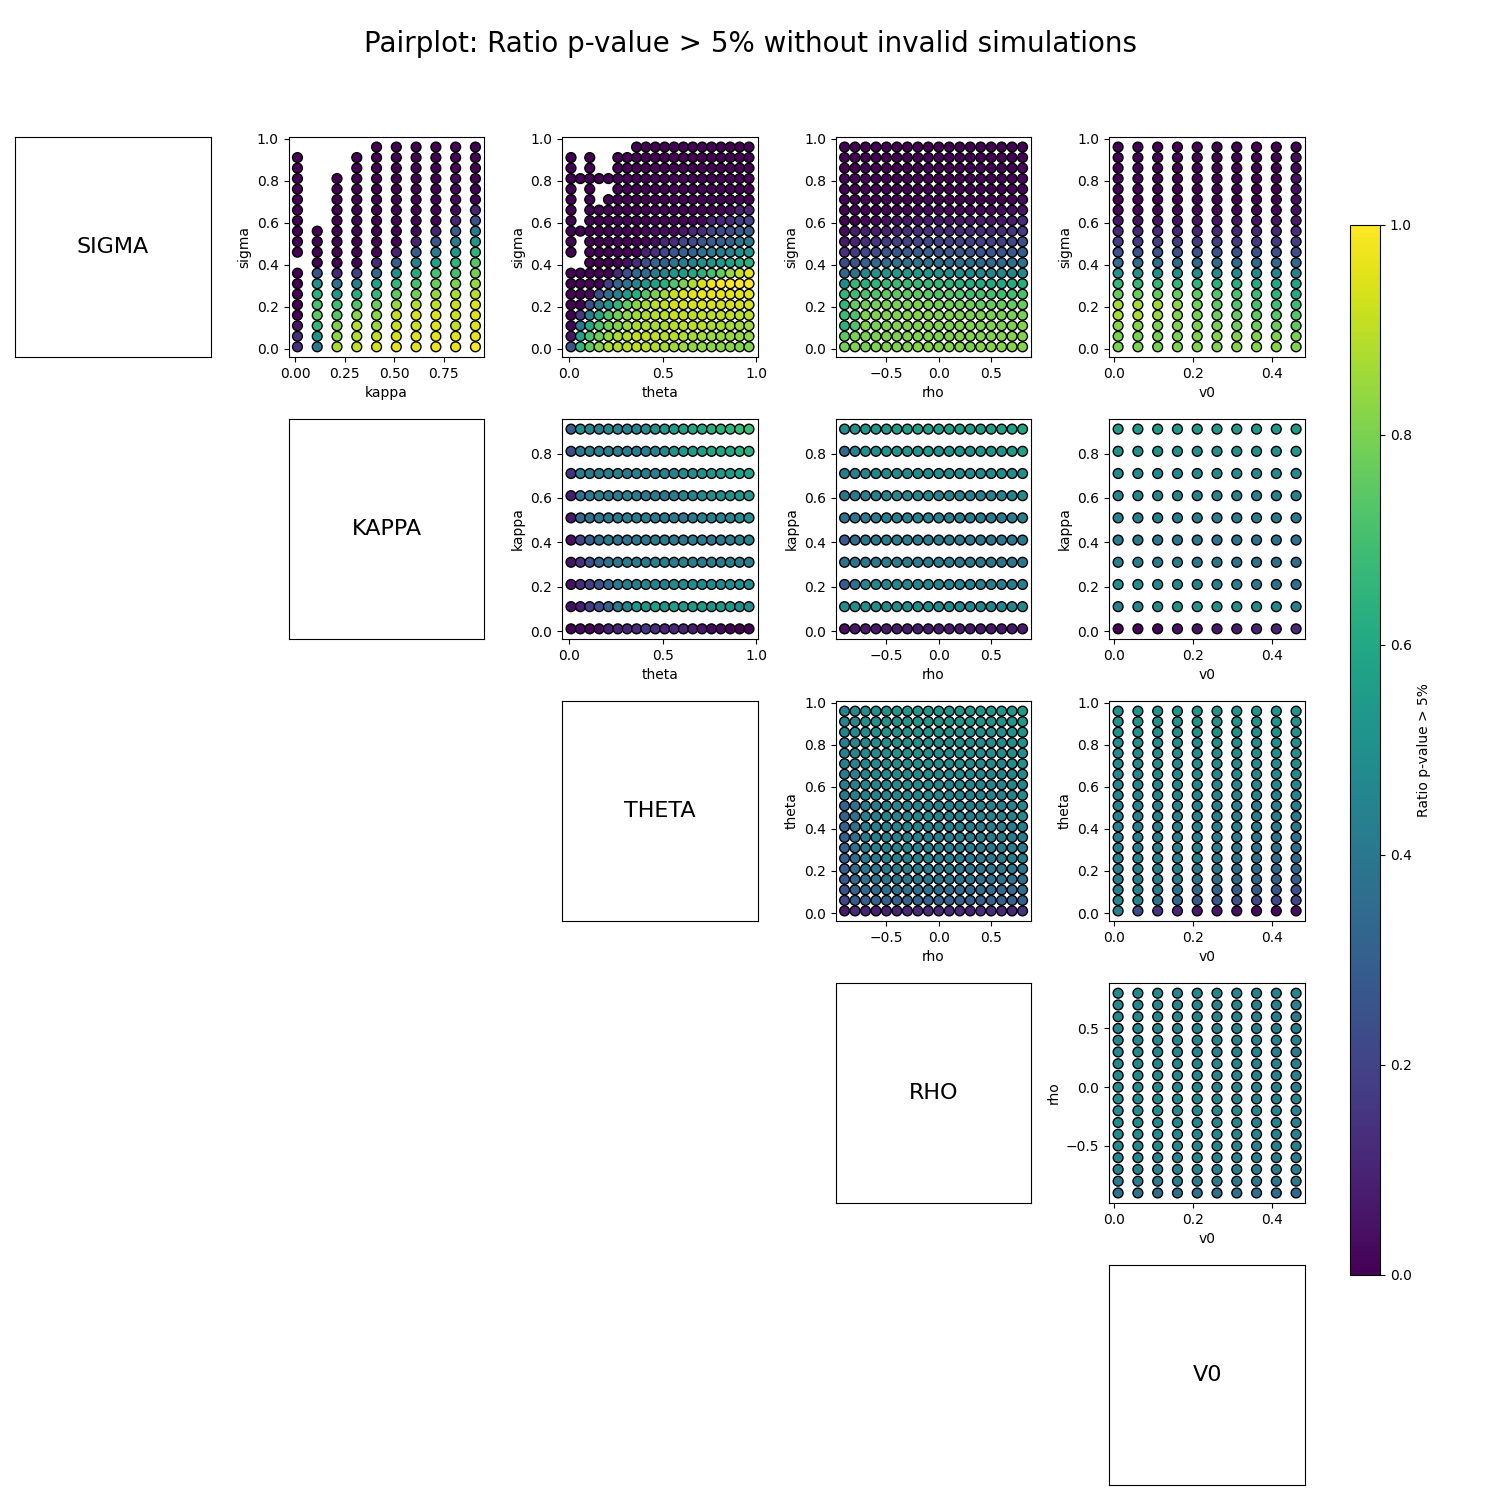
\includegraphics[width=0.8\textwidth]{img/pairplot_GC_cum_AD.png}
    \caption{Pairplot for each pair of parameters for the Heston Model and the percentage of p values of the Anderson-Darling-Test for the Gram-Charlier Expansion with Cumulants vs the theoretical density above 5\%. Invalid simulations are excluded and $\mu=0.05$.}
    \label{fig:pairplot_GC_cum_AD_mu005}
\end{figure}
\chapter{Conclusion and Future Work}
\label{sec:conclusion_future_work}

- Die numerischen Fehler während der Simulation des Heston-Models mittels QE-Schema konnten identifiziert und ausgeschlossen werden. Es stellte sich heraus, dass, wenn die Feller condition zu stark nicht erfüllt war, diese Fehler auftauchten. Andersen (2008) schreibt aber in seinem Paper, dass das QE-Schema auch in solchen Fällen funktioniert, es kann sich also nur um einen Fehler in der Implementierung handeln. Tatsächlich konnte dieser Fehler zum Ende dieser Arbeit gefunden und behoben werden, die Zeit reichte aber nicht mehr aus, um diese Simulationen neu durchrechnen zu lassen. Problem war die Berechnung der Gleichung \eqref{eq:qe_dirac} und das Ziehen von $U_v$ aus der uniform distribution. Falls $U_v$ dort exakt den Wert 1 annimmt, so wird zur Berechnung von $\Psi^{-1}$ durch 0 geteilt, was zu dem Fehler führt. Das kommt aber nur zum Tragen, wenn $v_t$ sehr klein ist und bleibt, also die Feller condition stark nicht erfüllt ist. Das Ziehen von $U_v$ wurde so angepasst, dass es zwischen $10^{-10}$ und $1-10^{-10}$ liegt. Einige kurze Tests haben gezeigt, dass dieser Fehler damit behoben ist.

% Festlegen des Bibliografie-Stils, in diesem Fall die deutsche Variante des Standard-Stils plain
% Für Bachelor- und Masterarbeiten sollte biblatex oder natbib verwendet werden. Eine kurze Suche bei Google führt auf die Paketdokumentationen,
% aus der sich alles Weitere ergibt.
% \bibliographystyle{gerplain}

% Einbinden der Bibliothek
\printbibliography
\thispagestyle{empty}

% Befehl zum Erstellen der Selbstständigkeitserklärung. Achtung: Es werden die Namen der Autoren, die in titlepage.tex festgelegt wurden, herangezogen und das Datum in \date{} verwendet.
% Befehl steht nur zur Verfügung, wenn das Paket VOSStatement eingebunden ist.
\cleardoublepage

\makestatement

% % % % % % % % % % % % % % % %
% Ende der document-Umgebung
% % % % % % % % % % % % % % % %
\end{document}